\documentclass[11pt]{aghdpl}
% \documentclass[en,11pt]{aghdpl}  % praca w języku angielskim

% Lista wszystkich języków stanowiących języki pozycji bibliograficznych użytych w pracy.
% (Zgodnie z zasadami tworzenia bibliografii każda pozycja powinna zostać utworzona zgodnie z zasadami języka, w którym dana publikacja została napisana.)
\usepackage[english,polish]{babel}

% Użyj polskiego łamania wyrazów (zamiast domyślnego angielskiego).
\usepackage{polski}

\usepackage[utf8]{inputenc}

% dodatkowe pakiety

\usepackage{mathtools}
\usepackage{amsfonts}
\usepackage{amsmath}
\usepackage{amsthm}
\usepackage{changepage}
% --- < bibliografia > ---

\usepackage[
style=numeric,
sorting=none,
%
% Zastosuj styl wpisu bibliograficznego właściwy językowi publikacji.
language=autobib,
autolang=other,
% Zapisuj datę dostępu do strony WWW w formacie RRRR-MM-DD.
urldate=iso,
seconds=true,
% Nie dodawaj numerów stron, na których występuje cytowanie.
backref=false,
% Podawaj ISBN.
isbn=true,
% Nie podawaj URL-i, o ile nie jest to konieczne.
url=false,
%
% Ustawienia związane z polskimi normami dla bibliografii.
maxbibnames=3,
% Jeżeli używamy BibTeXa:
backend=bibtex
]{biblatex}
\usepackage{csquotes}
% Ponieważ `csquotes` nie posiada polskiego stylu, można skorzystać z mocno zbliżonego stylu chorwackiego.
\DeclareQuoteAlias{croatian}{polish}

\addbibresource{bibliografia.bib}

% Przecinki zamiast kropek do oddzielenia pól wpisu bibliograficznego
% i dwukropek po nazwisku autora, bez kropki na końcu
\AtBeginBibliography{
    \renewcommand\labelnamepunct{:\space}
    \renewcommand\newunitpunct{\addcomma\space}
    \renewcommand{\finentrypunct}{}

    \renewcommand{\bibopenparen}{\addcomma\addspace}
    \renewcommand{\bibcloseparen}{\addspace}
}


% Nie wyświetlaj wybranych pól.
%\AtEveryBibitem{\clearfield{note}}


% ------------------------
% --- < listingi > ---

% Użyj czcionki kroju Courier.
\usepackage{courier}

\usepackage{listings}
\lstloadlanguages{TeX}

\lstset{
	literate={ą}{{\k{a}}}1
           {ć}{{\'c}}1
           {ę}{{\k{e}}}1
           {ó}{{\'o}}1
           {ń}{{\'n}}1
           {ł}{{\l{}}}1
           {ś}{{\'s}}1
           {ź}{{\'z}}1
           {ż}{{\.z}}1
           {Ą}{{\k{A}}}1
           {Ć}{{\'C}}1
           {Ę}{{\k{E}}}1
           {Ó}{{\'O}}1
           {Ń}{{\'N}}1
           {Ł}{{\L{}}}1
           {Ś}{{\'S}}1
           {Ź}{{\'Z}}1
           {Ż}{{\.Z}}1,
	basicstyle=\footnotesize\ttfamily,
}

% ------------------------

\AtBeginDocument{
	\renewcommand{\tablename}{Tabela}
	\renewcommand{\figurename}{Rys.}
}

% ------------------------
% --- < tabele > ---

\usepackage{array}
\usepackage{tabularx}
\usepackage{multirow}
\usepackage{booktabs}
\usepackage{makecell}
\usepackage[flushleft]{threeparttable}
\usepackage{hyperref}

% defines the X column to use m (\parbox[c]) instead of p (`parbox[t]`)
\newcolumntype{C}[1]{>{\hsize=#1\hsize\centering\arraybackslash}X}


%---------------------------------------------------------------------------

\author{inż. Małgorzata Szwed}
\shortauthor{M. Szwed}

%\titlePL{Przygotowanie bardzo długiej i pasjonującej pracy dyplomowej w~systemie~\LaTeX}
%\titleEN{Preparation of a very long and fascinating bachelor or master thesis in \LaTeX}

\titlePL{Detekcja anomalii w sygnale mowy u osób z chorobą Parkinsona}
\titleEN{Anomalies detection in speech signals in people with Parkinson's disease}


\shorttitlePL{Detekcja anomalii w sygnale mowy u osób z chorobą Parkinsona} % skrócona wersja tytułu jeśli jest bardzo długi
\shorttitleEN{Anomalies detection in speech signals in people with Parkinson's disease}

\thesistype{Praca dyplomowa}
%\thesistype{Master of Science Thesis}

\supervisor{dr inż. Daria Hemmerling}

\degreeprogramme{Inżynieria Biomedyczna}
%\degreeprogramme{Computer Science}

\date{2023}

%\department{Katedra Informatyki Stosowanej}
%\department{Department of Applied Computer Science}

\faculty{Wydział Elektrotechniki, Automatyki,\protect\\[-1mm] Informatyki i Inżynierii Biomedycznej}
%\faculty{Faculty of Electrical Engineering, Automatics, Computer Science and Biomedical Engineering}

\acknowledgements{Chciałbym serdecznie podziękować mojej pani promotor, dr inż. Darii Hemmerling, za okazane wspracie, inspirację i bezstresową atmosferę.
Dziękuję również wszystkim zaangażowanym w proces zbierania nagrań, za Wasz nieoceniony wkład w rozwój nauki.}

\setlength{\cftsecnumwidth}{10mm}

%---------------------------------------------------------------------------
\setcounter{secnumdepth}{4}
\brokenpenalty=10000\relax

% rubber: bibtex.path ./

\begin{document}

\titlepages

% Ponowne zdefiniowanie stylu `plain`, aby usunąć numer strony z pierwszej strony spisu treści i poszczególnych rozdziałów.
\fancypagestyle{plain}
{
	% Usuń nagłówek i stopkę
	\fancyhf{}
	% Usuń linie.
	\renewcommand{\headrulewidth}{0pt}
	\renewcommand{\footrulewidth}{0pt}
}

\setcounter{tocdepth}{1}
\tableofcontents
\clearpage

\chapter{Wprowadzenie} \label{ch:wprowadzenie}

Choroba Parkinsona (ang. \emph {Parkinson Disease, PD}) to zwyrodnieniowe schorzenie mózgu, które wiąże się z objawami ruchowymi, takimi jak spowolnienie ruchowe,
drżenie, sztywność oraz zaburzenia chodu i równowagi.
Ponadto może prowadzić do różnorodnych powikłań niemotorycznych, obejmujących zaburzenia poznawcze, stany psychiczne,
trudności ze snem oraz dolegliwości sensoryczne, w tym ból.
Początkowe objawy często rozwijają się stopniowo, nasilając się w miarę upływu czasu.
Postęp choroby prowadzi do znacznego stopnia niepełnosprawności, co może wymagać wsparcia i opieki.
U wielu osób zdiagnozowanych z chorobą Parkinsona występują także zmiany w sferze psychicznej i behawioralnej, takie jak
trudności ze snem, depresja, problemy z pamięcią oraz uczucie przewlekłego zmęczenia.

\begin{figure}[htbp]
	\centering
	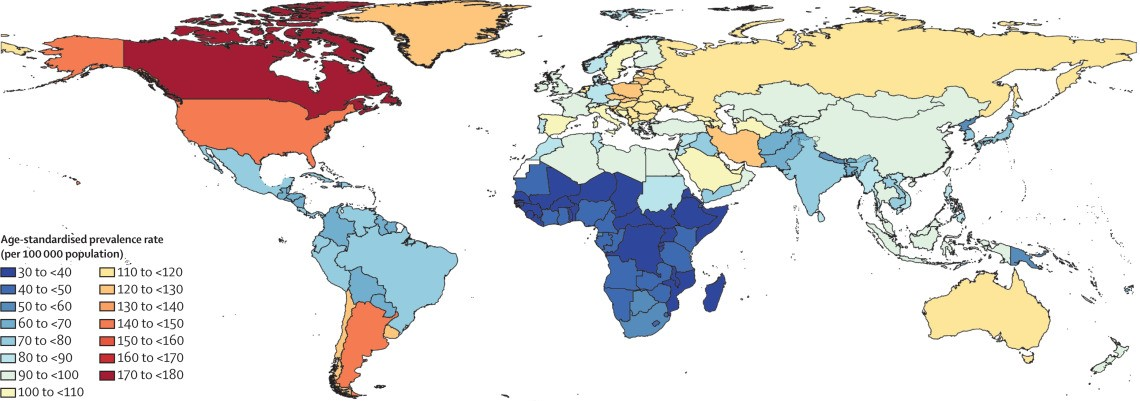
\includegraphics[width=0.9\textwidth]{./img/map}
	\caption{Choroba Parkinsona na świecie~\cite {global_PD}}
    \label{fig:PD_map}
\end{figure}

Zgodnie z danymi przedstawionymi w raporcie Światowej Organizacji Zdrowia~\cite{WHO}, choroba Parkinsona stanowi obecnie narastający problem na skalę światową.
Zarówno wskaźniki niepełnosprawności, jak i zgony związane z tą chorobą rosną szybciej niż w przypadku innych zaburzeń neurologicznych.

W ciągu ostatnich 25 lat zaobserwowano podwojenie częstości występowania PD na całym świecie.
Globalne szacunki na rok 2019 wskazują, że liczba osób cierpiących na PD przekroczyła 8,5 miliona, co oznacza wzrost o 81\% w porównaniu z danymi z roku 2000.
Jednocześnie liczba zgonów związanych z PD wyniosła 329~000, co stanowi wzrost o ponad 100\% w porównaniu z rokiem 2000\cite{global_PD}.
W Polsce z chorobą Parkinsona zmaga się około 100 tys.
pacjentów, z czego około 20\% jest już w stadium zaawansowanym
według informacji przekazywanych przez Fundację Chorób Mózgu.
Ponadto co roku w naszym kraju wykrywanych jest ok.
8 tys.
nowych zachorowań.

PD jest istotną sprawą dotyczącą zdrowia publicznego, ponieważ jej częstotliwość występowania związana jest ze zjawiskiem starzejącego się społeczeństwa (Rys.~\ref{fig:PD_map}).
Razem z innymi chorobami neurodegeneracyjnymi, takimi jak choroba Alzheimera, ma szanse stać się drugą zaraz za nowotworami przyczyną zgonów do 2040 roku (WHO).

Przyczyna PD nie jest znana, ale uważa się, że powstaje w wyniku złożonej interakcji pomiędzy czynnikami genetycznymi i
narażeniem na czynniki środowiskowe, takie jak pestycydy, rozpuszczalniki i zanieczyszczenia powietrza.
Niektóre przypadki wydają się dziedziczne, a kilka można przypisać określonym wariantom genetycznym.
Chociaż uważa się, że genetyka odgrywa rolę w chorobie Parkinsona, w większości przypadków choroba nie występuje rodzinnie\cite{National_Institute_on_Aging_2022}.

\begin{figure}[htbp]
	\centering
	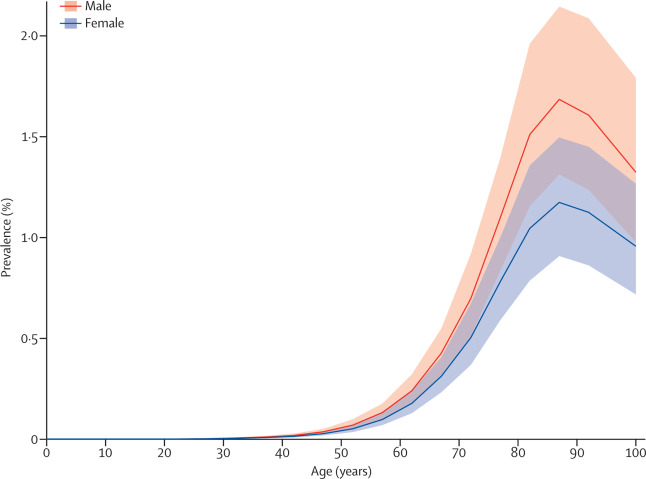
\includegraphics[width=0.5\textwidth]{./img/PD_prevalence}
	\caption{Rozpowszechnienie choroby Parkinsona w zależności od wieku \cite {global_PD}}
    \label{fig:PD_prevalance}
\end{figure}

Mimo że każdy może być narażony na ryzyko rozwoju tej choroby, to częściej występuje ona u mężczyzn niż u kobiet,
a wiek stanowi kluczowy element wpływający na ryzyko zachorowania, co można zobaczyć na Rys.\ref{fig:PD_prevalance}.
Statystyki pokazują, że ryzyko zachorowania rośnie wraz z wiekiem, chociaż choroba może dotyczyć także młodszych osób (nawet w wieku 20 lat).
U większości pacjentów po raz pierwszy choroba rozwija się po 60 roku życia, około 5\% do 10\% doświadcza jej początku przed 50 rokiem życia.
Postacie choroby Parkinsona o wczesnym początku są często, choć nie zawsze, dziedziczne i niektóre formy zostały powiązane z
określonymi zmianami w genach\cite{National_Institute_on_Aging_2022}.

Proces diagnozowania choroby jest niezwykle złożony i czasochłonny, nie istnieje obecnie pojedyncze badanie pozwalające na postawienie diagnozy.
W związku z tym poszukuje się nowych rozwiązań, które mogłyby usprawnić ten proces.
Coraz częściej wykorzystuje się metody uczenia maszynowego i sztucznej inteligencji w dziedzinie medycyny.
W niniejszej pracy analizowany jest aktualny stan rzeczy oraz przedstawiane jest proponowane rozwiązanie, dotyczące automatycznej diagnostyki
choroby Parkinsona na podstawie głosu.

%---------------------------------------------------------------------------

\section{Cel pracy}
\label{sec:celPracy}

Celem pracy jest detekcja choroby Parkinsona na podstawie sygnału głosowego z wykorzystaniem metod uczenia maszynowego.
Obejmuje to dokładny przegląd literaturowy ze szczególnym uwzględnieniem aktualnie najlepszych algorytmów
dostępnych w literaturze.
Pośrednim celem jest ocena skuteczności wybranych architektur konwolucyjnych sieci neuronowych (CNN) oraz analiza, która z wypowiadanych przez
pacjentów samogłosek niesie ze sobą najwięcej informacji diagnostycznej.

%---------------------------------------------------------------------------

\section{Zakres pracy}
\label{sec:zakresPracy}

\chapter{Problematyka zagadnienia}
\label{ch:problematyka}

%---------------------------------------------------------------------------

\section{Znaczenie głosu w chorobie Parkinsona}
\label{sec:znaczenie_glosu}

Najbardziej widoczne oznaki i objawy choroby Parkinsona pojawiają się, gdy komórki nerwowe w zwojach podstawy mózgu,
obszarze kontrolującym ruch, ulegają uszkodzeniu i/lub obumierają.
Zwykle te komórki nerwowe lub neurony wytwarzają dopaminę.
Kiedy neurony obumierają lub ulegają uszkodzeniu, wytwarzają mniej dopaminy, co powoduje problemy z poruszaniem się
związane z chorobą.
Na ten moment nie wiadomo co powoduje śmierć neuronów.
Zanikają również zakończenia nerwowe, które wytwarzają norepinefrynę, główny przekaźnik chemiczny
współczulnego układu nerwowego, który kontroluje wiele funkcji organizmu, takich jak tętno i ciśnienie krwi.
Utrata norepinefryny może pomóc wyjaśnić niektóre cechy choroby Parkinsona związane z brakiem ruchu, takie jak zmęczenie,
nieregularne ciśnienie krwi, zmniejszony ruch pokarmu w przewodzie pokarmowym i nagły spadek ciśnienia krwi, gdy osoba wstaje z pozycji siedzącej lub leżącej.

\vspace{0.5cm}
Do czterech głównych objawów choroby Parkinsona zalicza się:
\begin{itemize}[itemsep=0.05pt]
	\item drżenie rąk, ramion, nóg, szczęki lub głowy,
	\item sztywność mięśni, gdy mięśnie pozostają skurczone przez długi czas,
	\item powolność ruchu,
	\item zaburzenia równowagi i koordynacji, czasami prowadzące do upadków.
\end{itemize}

Zarówno objawy choroby Parkinsona jak i tempo jej postępu mogą znacząco różnić się wśród poszczególnych osób.
Na wczesnym etapie choroby objawy są subtelne i kształtują się stopniowo.
Często zaczynają się od jednej strony ciała lub nawet jednej kończyny.
Niektórzy pacjenci doświadczają pewnych zwiastunów przed wystąpieniem charakterystycznych cech, takich jak sztywność czy drżenie.
Mogą to być trudności ze snem, problemy z wypróżnianiem, utrata węchu czy także zespół niespokojnych nóg.
Warto jednak zaznaczyć, że niektóre z wymienionych objawów mogą również występować w procesie naturalnego starzenia się \cite{National_Institute_on_Aging_2022}.

Chociaż tempo postępu choroby Parkinsona zazwyczaj jest powolne, w końcu ma to wpływ na codzienne funkcjonowanie osoby dotkniętej tą dolegliwością.
Wykonywanie zwykłych czynności, takich jak praca, prowadzenie domu czy uczestnictwo w spotkaniach towarzyskich z przyjaciółmi, może stawać się wyzwaniem.

Choroba Parkinsona jest spowodowana zaburzeniem funkcji układu nerwowego, co prowadzi do występowania objawów w różnych obszarach organizmu, w tym również w sferze głosu.
Objawy zaburzeń mowy dotyczą między 60 a 80\% pacjentów, a powodowane są przede wszystkim przez deficyt czynnościowy krtani,
zmniejszoną pojemność życiową płuc, osłabioną pracę mięśni mimicznych oraz zmiejszony napęd mówienia \cite{lewicka}.
Zwykle stają się widoczne w średniozaawansowanym stadium schorzenia, co oznacza, że przez długi okres mowa pozostaje relatywnie nienaruszona.
Rozpoznanie tych zaburzeń może być niekiedy trudne, gdyż wymaga odróżnienia, czy powstały one na skutek samej choroby, czy też są rezultatem naturalnego
procesu starzenia się organizmu.

Objawy zaburzeń mowy i głosu związane z chorobą Parkinsona nie są łatwo dostrzegalne dla osób bez specjalistycznej wiedzy w tej dziedzinie.
Przeważnie zdolność rozumienia mowy pozostaje niezmieniona.
Niemniej jednak, w trakcie spontanicznych wypowiedzi pacjenci zaczynają ograniczać ilość przekazywanych informacji i mogą napotykać trudności w składaniu
pełnych zdań.
Trudności te nie wynikają koniecznie z ubytku słownictwa, ale raczej z nieprawidłowego doboru słów.
Wskazujące na podłoże chorobowe objawy obejmują między innymi \cite{Szurek_2018, Kuryłowicz_2019}:
\begin{itemize}[itemsep=0.1pt]
	\item mowę powolną, monotonną i przerywaną,
	\item nadmierne ślinienie się,
	\item niewyraźną i zamazaną artykulację,
	\item skrócony czas fonacji
	\item chuchający i tremolujący głos
	\item spłaszczoną barwę i obniżone natężenie
	\item niewłaściwą koordynację mięśni nasady, które mogą być zwiotczałe lub zbyt napięte,
	\item czasami przyspieszenie tempa wypowiedzi w jej końcowej fazie, co może utrudnić zrozumienie pacjenta.
\end{itemize}

Wymienione objawy pojawiają się w średniozaawansowanym stadium choroby i są wystarczająco wyraźne, aby mogły zostać zauważone słuchowo przez specjalistów.
Niemniej jednak badania wskazują, że istnieją subtelne zmiany w głosie, które pojawiają się jeszcze wcześniej, nawet w fazie przedobjawowej \cite{2023_PD_voice}.

W roku 2000 przeprowadzono badanie akustyczne i percepcyjne cech głosu pacjentów z chorobą Parkinsona, zależnie od stopnia nasilenia choroby \cite{https://doi.org/10.1080/136828200410654}.
W nagraniach głosowych, składających się z przedłużonej samogłoski /a/, śpiewu gamy oraz 1-minutowego monologu, stwierdzono, że głosy pacjentów z PD,
zarówno we wczesnych, jak i późniejszych stadiach choroby, charakteryzowały się ograniczoną percepcyjnie zmiennością tonu i głośności, chropowatością
oraz zmniejszoną głośnością.

Badanie sugerowało również, że głosy pacjentów z PD wykazywały nadmierne drganie, wysoką częstotliwość podstawową (szczególnie u mężczyzn) oraz zmniejszoną zmienność częstotliwości podstawowej (szczególnie u kobiet).
Część z tych cech głosu nie wydawała się pogarszać w miarę postępu choroby, jednak cechy takie jak oddech, monotonność i jednolitość mowy, niska głośność oraz ograniczony maksymalny zakres częstotliwości fonacyjnej były bardziej zauważalne w późniejszych stadiach choroby Parkinsona.

Podobne badanie przeprowadzone przez Gamboę i innych (1997) wykazało, że w porównaniu z grupą kontrolną, pacjenci z PD wykazywali wyższy jitter, niższy
stosunek harmonicznych do szumów (H/N), mniejszą zmienność częstotliwości i intensywności mowy oraz niższy zakres fonacyjny oraz wyższą częstotliwość
obecności głosu o niskim natężeniu.
Wskazano również, że te cechy nie wykazywały znaczącego związku z czasem trwania choroby \cite{GAMBOA1997314}.

Mnogość objawów, które są zauważalne w głosie, motywuje do uzwględnienia ich w diagnostyce.
Prowadzone są badania, które wykorzystują analizę mowy do wykrywania patologii i schorzeń związanych z narządem głosu, takich jak ostre zapalenie krtani czy porażenie nerwu krtaniowego wstecznego.
Może to w przyszłości pozwolić na identyfikację problemów zdrowotnych, na przykład wśród osób pracujących głosem, jak nauczyciele, bez konieczności inwazyjnych badań gardła.
Podobne podejście można zastosować do diagnozowania i monitorowania chorób neurodegeneracyjnych.
Badania naukowe wskazują, że analiza głosu może stanowić podstawę dla automatycznej diagnostyki oraz monitorowania choroby Parkinsona.

Takie podejście niesie ze sobą wiele korzyści, które mogą rewolucjonizować sposób diagnozowania oraz monitorowania tej neurodegeneracyjnej choroby.
Głos, będący wskaźnikiem stanu układu nerwowego i zdolności komunikacyjnych, dostarcza szeroką gamę informacji kluczowych dla procesu diagnozowania.
Różnorodność parametrów akustycznych i fonacyjnych, które można zbadać, otwiera drzwi do kompleksowej oceny zmian zachodzących w organizmie pacjenta.

Wczesne objawy choroby Parkinsona często bywają trudne do wykrycia, szczególnie w standardowych badaniach klinicznych.
Analiza głosu pozwala na szybką identyfikację subtelnych zmian, które pojawiają się we wczesnych fazach choroby.
Ta wczesna detekcja umożliwia natychmiastową interwencję terapeutyczną, co może wpłynąć na spowolnienie progresji choroby i poprawę jakości życia pacjenta.

Analiza głosu jako narzędzie diagnostyczne wprowadza nowe perspektywy dla specjalistów zajmujących się chorobą Parkinsona.
Logopedzi, foniatrzy i lekarze mogą wykorzystać obiektywne dane akustyczne do dokładnej oceny zmian w mowie i jakości głosu pacjenta.
To również umożliwia sugerowanie odpowiednich interwencji, włącznie z dostosowaniem leczenia farmakologicznego.

Dla pacjentów oznacza to bardziej konkretne oceny ich stanu i dostosowane terapie, przyczyniające się do zwiększenia efektywności procesu leczenia.
Badanie to jest szybkie, wygodne i bezpieczne, co może zachęcać pacjentów do systematycznego uczestnictwa w procesie diagnostycznym.
Wprowadza to szczególną wartość dla pacjentów, którym trudno się przemieszczać.

Analiza głosu jako narzędzie diagnostyczne przy chorobie Parkinsona otwiera drzwi ku nowym, zaawansowanym metodologiom diagnozowania i leczenia.
Może być wykorzystana do oceny stanu pacjenta oraz sugerowania odpowiednich interwencji, włączając zmiany w leczeniu farmakologicznym.
W konsekwencji ma potencjał stania się szybkim, nieinwazyjnym wsparciem diagnostycznym i terapeutycznym, przyczyniając się do polepszenia
opieki nad pacjentami dotkniętymi chorobą Parkinsona.

%---------------------------------------------------------------------------
\section{Metody diagnozowania i monitorowania}
\label{subsec:diagnostyka}

Diagnostyką choroby Parkinsona zajmują się neurolodzy i geriatrzy.
Rozwój PD jest długotrwały, a w początkowych latach klinicznie niemal niewidoczny, co utrudnia wczesne rozpoznanie.
Subtelne objawy często są uważane za skutek starzenia się lub błędnie diagnozowane jako inne zaburzenia neurologiczne.
Kluczowym elementem w tym stadium jest dokładny wywiad, badanie fizykalne oraz identyfikacja objawów przez lekarza.
Następnie diagnoza jest rozwijana poprzez badania laboratoryjne  oraz obrazowe.
Niestety, wyniki tych badań rzadko potwierdzają diagnozę od razu.

Początkowo pacjent zwykle konsultuje się z lekarzem pierwszego kontaktu, który powinien dokonać wstępnej diagnozy i skierować do neurologa.
W tej fazie diagnozy przeprowadza się szczegółowy wywiad, uwzględniający rodzaj, nasilenie oraz okres występowania objawów, a także
obecność chorób neurozwyrodnieniowych w rodzinie.
Neurolog przeprowadza kompleksowe badanie neurologiczne, identyfikując symptomy takie jak sztywność mięśni, ograniczenia w
ruchu (spowolnienie, trudności w poruszaniu się), drżenia spoczynkowe (np. w głowie, palcach rąk) oraz zaburzenia postawy i równowagi
(zgarbienie, niestabilność, upadki). Kolejne badania są wykonywane w celu potwierdzenia lub wykluczenia diagnozy \cite{diagnostyka_Sitek, Loscalzo_2022}.

\renewcommand{\labelenumi}{\alph{enumi})}
\begin{enumerate}
	\item Badania laboratoryjne
	\item[] Obecnie brak specyficznych badań laboratoryjnych krwi, które potwierdzałyby diagnozę choroby Parkinsona.
Niemniej jednak, takie badania są użyteczne w wykluczaniu innych chorób o podobnym przebiegu.
Wykonuje się podstawowe badania, takie jak morfologia krwi, elektrolity, poziom glukozy, TSH, próby wątrobowe, mocznik, kreatynina oraz poziom witaminy B12.

	\item Badania obrazowe
	\item[] Badania obrazowe głowy są przeprowadzane w celu wykluczenia innych chorób o podobnych objawach.
Zalicza się do nich tomografię komputerową, ultrasonografię mózgu (USG) oraz rezonans magnetyczny głowy (MRI).
Międzynarodowe kryteria rozpoznania choroby Parkinsona nie nakładają obowiązku wykonywania badań obrazowych w celu potwierdzenia diagnozy.
Dostępne są również zaawansowane techniki obrazowania, takie jak PET (pozytonowa emisyjna tomografia) oraz SPECT (tomografia emisyjna pojedynczego fotonu), które pozwalają na obserwację metabolizmu w układzie pozapiramidowym. Skan DAT (skan transportera dopaminy) jest przykładem SPECT i może być sugerowany przez specjalistę.
Mimo to, ostateczna diagnoza opiera się na objawach oraz wynikach badania neurologicznego. Większość pacjentów nie wymaga skanowania DAT.

	\item Test z lewodopą
	\item[]Test polega na podaniu pacjentowi  preparatu z lewodopą.
Jeśli następuje poprawa po zażyciu, istnieje wysokie prawdopodobieństwo, że pacjent rzeczywiście cierpi na chorobę Parkinsona.
W przypadku braku poprawy, konieczne może być dalsze rozszerzenie diagnostyki.

	\item Badania genetyczne
	\item[] Choroba Parkinsona może występować rodzinnie, co skłania do rozważenia diagnostyki genetycznej u pacjenta i jego krewnych.
Obecnie zidentyfikowano 12 mutacji genów, które mogą wpływać na ryzyko zachorowania na PD, należy jednak pamiętać, że badania genetyczne są kosztowne.

	\item Badania węchu
	\item[] Większość osób z chorobą Parkinsona (90\%) doświadcza zaburzeń węchu, manifestujących się hiposomią (osłabienie węchu), także we wczesnym stadium choroby.
Jednak nie obserwuje się tych zaburzeń w przypadku zaniku wieloukładowego i postępującego porażenia nadjądrowego.

	\item Badania neuropsychologiczne i neuropsychiatryczne
	\item[] Badania te służą identyfikacji zaburzeń poznawczych i emocjonalnych.
Celem jest diagnoza łagodnych zaburzeń poznawczych, otępienia, a także zaburzeń psychotycznych, lękowych, kontroli impulsów i depresji.
\end{enumerate}

Objawy przypominające chorobę Parkinsona są diagnozowane jako parkinsonizm i mogą być spowodowane różnymi zaburzeniami, takimi jak postępujące porażenie nadjądrowe, zanik wieloukładowy,
drżenie samoistne, demencja z ciałami Lewy'ego, choroby naczyniowe mózgu, otępienie, reumatyzm i inne \cite{diagnostyka_Sitek}.
Różnicowanie tych schorzeń jest kluczowe, ponieważ leczenie i podejście terapeutyczne są różne.
Chociaż ostateczną diagnozę można ustalić tylko na podstawie badania mózgu po zgonie, wcześniej zdefiniowane kryteria diagnostyczne pozwalają na dokonanie diagnozy klinicznej.
Według badania z 2021 roku opisanego w publikacji \cite{ROSSI202153} diagnoza klinicznie potwierdzonej choroby Parkinsona może zabierać od kilku miesięcy do kilku lat, zależnie od indywidualnych czynników oraz reakcji na terapię lewodopą.
Uznaje się, że aktualnie wykorzystywane kryteria pozwalają na diagnozę z dokładnością 90\%, ale trwa to średnio 2,9 roku.

Pomocnym narzędziem w diagnostyce są szeroko stosowane skale oceny choroby Parkinsona.
Stanowią istotne narzędzie w monitorowaniu stanu pacjentów oraz pomagają lekarzom i opiekunom ocenić stopień nasilenia objawów ruchowych,
jak również wpływ choroby na codzienne funkcjonowanie pacjenta.
Popularne skale, takie jak Skala Hoehn-Yahra, Skala UPDRS (Unified Parkinson's Disease Rating Scale) oraz Skala Schwab-England,
umożliwiają stosunkowo obiektywną analizę symptomów i wsparcie w podejmowaniu decyzji terapeutycznych.
Dzięki tym narzędziom możliwe jest dostosowanie leczenia do indywidualnych potrzeb pacjenta oraz śledzenie skuteczności terapii na przestrzeni czasu.

Obecnie proces diagnozy jest wyjątkowo złożony i wieloetapowy.
W odpowiedzi na te wyzwania, naukowcy koncentrują się na opracowaniu bardziej efektywnych narzędzi diagnostycznych.
Rozwinięcie skuteczniejszych narzędzi diagnostycznych przyniesie korzyści nie tylko finansowe, ale także pozwoli na szybsze i trafniejsze udzielanie pomocy pacjentom.
W nadchodzących latach, dążenie do wypracowania bardziej efektywnych metod diagnozowania choroby Parkinsona będzie kluczowym krokiem w zapewnieniu lepszej opieki zdrowotnej i poprawie jakości życia pacjentów.

%---------------------------------------------------------------------------

\section{Terapia osób chorych}
\label{sec:terapia}
Obecnie brak jest kuracji na chorobę Parkinsona, dlatego terapia skupia się na przywracaniu pacjentom zdolności funkcjonowania
lub, w przypadkach zaawansowanych, na poprawie jakości życia.
Zgodnie z aktualnym standardem medycznym, w terapii wykorzystuje się różnorodne metody, w tym leczenie farmakologiczne, głęboką stymulację mózgu oraz rehabilitację \cite{National_Institute_on_Aging_2022}.

Leczenie farmakologiczne choroby Parkinsona opiera się na zwiększeniu poziomu dopaminy w mózgu, co wpływa na kontrolę objawów
ruchowych i niezwiązanych z ruchem. Główną terapią jest lewodopa, która jest przetwarzana przez komórki nerwowe w dopaminę.
Leczenie lewodopą często łączy się z karbidopą, która zmniejsza skutki uboczne i ilość potrzebnej lewodopy.
Stosuje się też inne terapie farmakologiczne o różnych zasadach działania m.in. pobudzające produkcję dopaminy,
zwiększające ilość dopaminy poprzez spowolnienie jej rozkładu, redukujące ruchy mimowolne czy zmniejszające drżenie i sztywność mięśni.

W przypadku pacjentów, u których leczenie farmakologiczne nie przynosi oczekiwanych efektów, może być rozważana Głęboka Stymulacja Mózgu (ang. \emph{Deep Brain Stimulation} - DBS).
W tym procederze chirurgicznym lekarz implantuje elektrody w określone obszary mózgu, łącząc je z małym urządzeniem elektrycznym umieszczonym w klatce piersiowej.
Poprzez bezbolesne stymulowanie konkretnych obszarów mózgu kontrolujących ruch, DBS może pomóc w zmniejszeniu wielu objawów związanych z ruchem,
takich jak drżenie, spowolnienie ruchu i sztywność.

Kluczową rolę w leczeniu odgrywa rehabilitacja neurologiczna, rozpoczynając się już od momentu postawienia diagnozy.
Jej wsparcie jest nieocenione w łagodzeniu zaburzeń chodu, głosu, drżenia, sztywności oraz pogorszenia funkcji umysłowych.
Wśród różnorodnych terapii, znajdują się między innymi:
\begin{itemize}[itemsep=0.1pt]
	\item zbilansowana dieta: wspiera ogólne samopoczucie pacjenta,
	\item ćwiczenia fizyczne: wzmacniają mięśnie, poprawiają równowagę, elastyczność i koordynację,
	\item masaż terapeutyczny: pomaga w redukcji napięcia mięśniowego oraz przynosi ulgę w objawach,
	\item joga i tai chi: wspomagają rozciąganie i elastyczność ciała, wpływając korzystanie na zdolność ruchową,
	\item rehabilitacja foniczna: pomaga w eliminowaniu trudności w mówieniu,
	\item psychoterapia: zapewnia wsparcie i umożliwia pacjentom pełne cieszenie się życiem pomimo choroby.
\end{itemize}


W ostatnim czasie na rynku pojawiło się też wiele aplikacji, które mają poprawić jakość życia osób z chorobą Parkinsona.
Na przykład, \emph{Parkinson's Central} zawierająca informacje dla pacjentów i opiekunów, obejmujące objawy, leczenie, wizyty lekarskie, zdrowy styl życia, badania i inne aspekty.
Podobną aplikacją jest \emph{Parkinson Symptom Tracker (PRO-PD App)}, zaprojektowana jako narzędzie do oceny i monitorowania nasilenia objawów choroby Parkinsona w czasie.
Bazuje na wywiadzie w formie testu, który umożliwia ocenę objawów.
Skala została opracowana w celu bycia wrażliwą na różne etapy choroby, charakteryzuje się dokładnością, szybkością, prostotą użycia i dostępnością.

Również w dziedzinie rehabilitacji ruchowej istnieje kilka aplikacji, takich jak \emph{Lift Pulse}, służąca do rejestrowania danych dotyczących drżenia rąk.
\emph{Delay the Disease}, czyli  program fitnessu rozwijany przez OhioHealth dla osób z chorobą Parkinsona, mający na celu poprawę funkcji fizycznych i opóźnienie postępu objawów choroby.
W kontekście rehabilitacji poprzez gry cyfrowe warto wspomnieć o platformie \emph{MindMotion® GO}.
Oferuje ona różnorodne aktywności i śledzenie ruchu ciała dzięki technologii śledzenia markerów.
Jedną z istotnych zalet programu to zdalne monitorowanie i dostosowanie przez terapeutę, zapewniające efektywną opiekę.

Obok aplikacji rehabilitacyjnych istnieje również \emph{Parkinson's Cognitive Research} dedykowana osobom zainteresowanym uczestnictwem w badaniach
naukowych dotyczących objawów poznawczych związanych z chorobą Parkinsona.
Aplikacja umożliwia analizę aspektów takich jak skupiona uwaga, percepcja wzrokowa, rozpoznawanie, pamięć krótkotrwała,
krótkotrwała pamięć wzrokowa, nazewnictwo, pamięć operacyjna, elastyczność poznawcza, planowanie, czas reakcji i prędkość przetwarzania.
Jej głównym celem jest wspieranie badań naukowych poprzez dostarczanie narzędzi cyfrowych do oceny i terapii poznawczej.
Mimo że stanowi cenny instrument dla społeczności naukowej oraz uniwersytetów na całym świecie, to jednak ma wyłącznie charakter badawczy i nie jest przeznaczona do diagnozowania ani leczenia choroby Parkinsona.

\subsection{Rola i zastosowanie aplikacji głosowych w poprawie jakości mowy u osób z chorobą Parkinsona}
\label{subsec:aplikacje-glosowe}

Tematem przewodnim tej pracy magisterskiej jest rola głosu w kontekście choroby Parkinsona. W związku z tym, przedstawione
zostaną różnorodne aplikacje dostępne obecnie na rynku, które koncentrują się na poprawie jakości głosu w przypadku tej choroby.

Jedną z nich jest \emph{Speak Up For Parkinson's}, przedstawiona przez Northwest Parkinson's Foundation.
Aplikacja skupia się szczególnie na głośności głosu pacjenta.
Oferuje dwa narzędzia do ćwiczeń: \emph{Słowa i Zwroty}, gdzie użytkownik musi wypowiedzieć serię losowych stwierdzeń oraz \emph{Czytanie i Konwersacja}, czyli obszar do swobodnych ćwiczeń o dłuższym czasie trwania.
W obu narzędziach dostarczany jest miernik głośności oraz opinie dźwiękowe/wideo.

Inną propozycją jest aplikacja \emph{Voice Trainer}, stworzona z myślą o osobach cierpiących na problemy z mową związane z chorobą Parkinsona,
ale również jest przydatna dla profesjonalnych mówców oraz, przy wsparciu logopedy, dla osób z innymi zaburzeniami głosu lub mowy.
W ramach aplikacji wyświetlane są wizualne informacje zwrotne dotyczące głośności i tonu mowy za pomocą jednej kropki na ekranie, co pozwala szybko
zidentyfikować obszary wymagające poprawy.
Aplikacja może być używana zarówno do ćwiczenia techniki, jak i do monitorowania toku rozmowy.

Kolejną godną uwagi aplikacją jest \emph{Delayed Auditory Feedback (DAF)}.
Przeznaczona jest dla osób z zaburzeniami mowy, które charakteryzują się szybkim tempem wypowiedzi.
Aplikacja pomaga użytkownikom zwolnić tempo mówienia, co w efekcie czyni je bardziej zrozumiałymi dla innych.
Działanie opóźnionej zwrotności dźwiękowej (DAF) polega na zmienionym odbiorze własnej mowy.
Zakłócenie normalnego cyklu zwrotnej informacji dźwiękowej skutkuje spowolnieniem tempa mówienia i poprawą klarowności wypowiedzi.

Aplikacja \emph{Beats Medical Parkinson's} objemuje rehabilitację objawów związanych z mową, chodem oraz drżeniem rąk.
Została zaprojektowana tak, aby pomóc użytkownikom ćwiczyć głośne i wyraźne mówienie, co przekłada się na większą pewność siebie podczas komunikacji.
Ważnym atutem aplikacji jest możliwość otrzymywania informacji zwrotnych w czasie rzeczywistym podczas ćwiczeń.
Dzięki temu użytkownicy mogą śledzić swoje postępy i dostosowywać trening do swoich potrzeb.

Aplikacja LSVT LOUD skupia się na treningu osób z chorobą Parkinsona w celu osiągnięcia bardziej naturalnego poziomu głośności podczas mówienia
w codziennych sytuacjach, takich jak komunikacja w domu, pracy czy w społeczności.
W kontekście teorii terapeutycznej, kluczowym aspektem tej metody jest pomoc pacjentom w "rekalibracji" ich percepcji dźwięku, aby byli świadomi
własnego głosu w kontekście interakcji z innymi ludźmi.
Dzięki tym treningom, osoby z chorobą Parkinsona mogą lepiej kontrolować swoją głośność mówienia i efektywniej uczestniczyć w komunikacji.

Zupełnie inną aplikacją, zapewniającą ciągłe wsparcie ze strony specjalistów jest \emph{Teleatherapy}.
Oferuje ona terapię głosu dla osób z chorobą Parkinsona.
Dzięki dostępowi zdalnemu pacjenci mogą oceniać swój stan oraz cele terapeutyczne, monitorować postępy i otrzymywać spersonalizowane wsparcie od logopedów.
Aplikacja kieruje użytkowników przez program terapii mowy, a ćwiczenia są dostosowane do indywidualnych potrzeb i przypisywane przez logopedę.
Ponadto terapeuci mają możliwość monitorowania ćwiczeń i udzielania opinii zwrotnej.

Aplikacja \emph{Voiceitt} nie ma zastosowania w rehabilitacji, ale możne znacznie poprawić komfort życia osób z chorobą Parkinsona.
Pomaga tłumaczyć niewyraźne lub nietypowe dźwięki na zrozumiałą mowę.
Każdy użytkownik trenuje oprogramowanie, podążając za prostymi komendami na ekranie.
Aplikacja może być zintegrowana jako samodzielne ASR (\emph{Automatic Speech Recognition}) dla osób o nietypowej mowie lub używany z innym systemem ASR
jako rozszerzenie dostępności z dodatkowym interfejsem dla osób z ograniczoną kontrolą ruchową i zaburzeniami mowy.
Planowane jest rozszerzenie aplikacji od napisów na spotkaniach po asystentów głosowych i sterowanie inteligentnym domem.

Powyższy przegląd ukazuje różnorodność dostępnych aplikacji, skierowanych do osób z chorobą Parkinsona.
Te narzędzia cyfrowe stanowią cenną pomoc dla pacjentów, jednak istotne jest zrozumienie, że nie zastępują one profesjonalnej terapii mowy prowadzonej
przez certyfikowanych logopedów.
Ich rola polega na ułatwianiu ćwiczeń i treningów, ale nie mogą pełnić funkcji zastępczej dla terapii specjalistycznych.
Warto zaznaczyć, że żadna z omówionych aplikacji nie posiada zdolności diagnostycznych.
Ich działanie opiera się na wsparciu w ćwiczeniach, terapii i monitorowaniu postępów, ale nie mają zdolności stawiania diagnoz.

Mimo tych ograniczeń, rosnące zainteresowanie dziedziną terapii mowy w kontekście choroby Parkinsona jest obiecujące.
Wspomniane aplikacje są dowodem na rozwijający się obszar badań i innowacji w tej dziedzinie.
W miarę postępu technologicznego istnieje szansa na powstanie nowych, bardziej zaawansowanych produktów, które mogą jeszcze skuteczniej wspomagać
osoby z chorobą Parkinsona w poprawie jakości mowy i komunikacji.

\chapter{Analiza rozwiązań do automatycznej diagnostyki choroby Parkinsona}\label{ch:analiza-rozwiazan}


Diagnoza PD jest powszechnie oparta na obserwacjach lekarskich i ocenie objawów klinicznych, w tym charakterystyce różnorodnych objawów ruchowych.
Rosnąca liczba zachorowań i obniżenie wieku osób będących w grupie ryzyka skutkuje wzrostem zainteresowania dotyczącym narzędzi, które ułatwiłyby
zarówno codzienne funkcjonowanie pacjentów, jak i pracę lekarzy.
Tradycyjne metody diagnostyczne mogą być obarczone subiektywizmem, ponieważ opierają się między innymi na ocenie ruchów, które są czasami subtelne dla
ludzkiego oka i dlatego trudne do sklasyfikowania, co może przyczynić się do błędnej diagnozy.
Ponadto wczesne objawy niemotoryczne PD mogą być łagodne oraz spowodowane wieloma innymi schorzeniami.
Dlatego też rozpoznanie tej choroby na wczesnym etapie stanowi wyzwanie.

Sztuczna inteligencja oraz nowoczesne technologie coraz częściej stają się integralną częścią systemu ochrony zdrowia.
Wspierają lekarzy podczas diagnozy oraz wyboru sposobu leczenia pacjenta, a także pozwalają na monitorowanie choroby.
Aby rozwiązać trudności i udoskonalić procedury diagnozowania oraz oceny PD, poszerzono stan techniki o metody uczenia maszynowego do
klasyfikacji PD i osób zdrowych lub pacjentów z podobnymi objawami klinicznymi (np.
zaburzeniami ruchu lub innymi zespołami parkinsonowskimi).
\section{Rodzaj wykorzystywanych danych}\label{sec:dane-przeglad}

Diagnozowanie choroby Parkinsona stanowi zadanie złożone ze względu na różnorodność objawów, które dotykają różnych aspektów
funkcjonowania ciała i umysłu ludzkiego.
W związku z tym, techniki uczenia maszynowego wykorzystywane w tym obszarze, także skupiają się na różnych rodzajach danych.
Wśród źródeł informacji diagnostycznej znajdują się wyniki badań obrazowych (np.
rezonans magnetyczny (MRI), tomografia komputerowa (SPECT)),
które wydają się intuicyjne, biorąc pod uwagę zmiany w aktywności mózgu, które można zaobserwować.
Niemniej jednak istnieją także mniej oczywiste metody diagnozy, które budzą duże zainteresowanie w środowisku naukowym, szczególnie w początkowym stadium choroby.
Przykłady to analiza głosu, ocena charakterystyki chodu oraz badanie pisma odręcznego.

\begin{figure}[htbp]
	\centering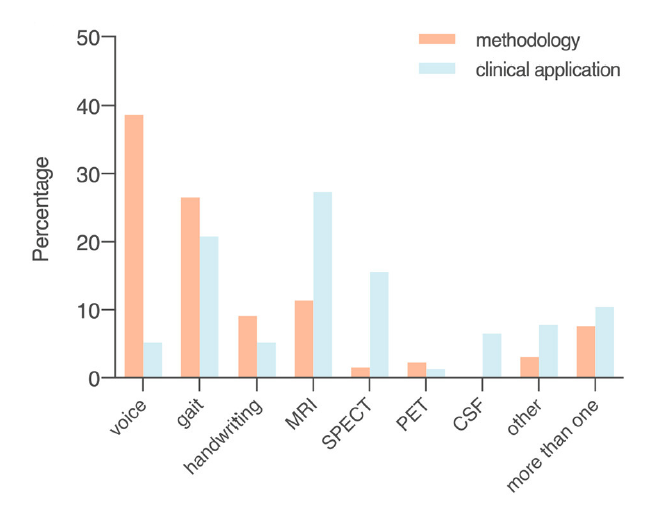
\includegraphics[width=0.6\textwidth]{./img/plot_PD_detection_methods}~\caption{Wykorzystanie rozwiązań w opracowaniach teoretycznych i zastosowaniach klinicznych w zależności od rodzaju danych (stan na 14 lutego 2020) \cite {ML_for_PD_review} }
    \label{fig:pd_detection_methods}
\end{figure}


Rys. \ref{fig:pd_detection_methods} ilustruje zastosowanie wymienionych metod zarówno w teorii, jak i praktyce.
Metody oparte na obrazowaniu medycznym wykazują wyraźną przewagę w zastosowaniach klinicznych w porównaniu do kontekstu teoretycznego.
Niemniej jednak to pozostałe metody budzą znacznie większe zainteresowanie ze strony środowiska naukowego.
Szczególnie w przypadku analizy głosu, gdzie rozbieżność między teorią a praktyką jest szczególnie znacząca.
Przyczyny tego zjawiska zostaną dokładniej rozważone w dalszej części pracy.
Co ciekawe, jak przedstawiono na Rys.~\ref{fig:pd_accuracy_methods}, detekcja choroby na podstawie głosu daje bardzo wysokie wyniki,
w większości analizowanych artykułów.

\begin{figure}[htbp]
	\centering
	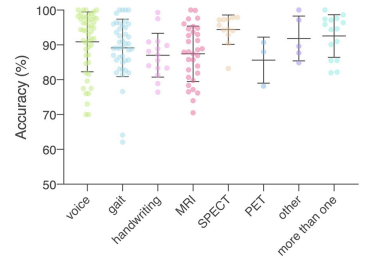
\includegraphics[width=0.6\textwidth]{./img/accuracy}~\caption{Dokładność rozwiązań diagnostycznych w zależności od rodzaju danych (stan na 14 lutego 2020) \cite {ML_for_PD_review} }
    \label{fig:pd_accuracy_methods}
\end{figure}

Niniejsza praca dotyczy diagnostyki opartej na analizie głosu, dlatego temat ten zostanie bliżej rozważony.
Założeniem dla takich systemów jest zadanie potencjalnemu pacjentowi zadania wokalnego, mogą to być:
\begin{itemize}[itemsep=0.1pt]
	\item podtrzymywane samogłoski (ang. \emph{sustained vowels}),
	\item zadanie diadochokinetyczne (DDK), mogące mierzyć zdolność do wydawania serii szybkich i naprzemiennych dźwięków (sylab),
	\item czytanie tekstu,
	\item wypowiedzenie pojedynczego zdania,
	\item monolog.
\end{itemize}

Dotychczas nie przeprowadzono badań porównawczych dotyczących wpływu wyboru zadania wokalnego na efektywność klasyfikacji w przypadku choroby Parkinsona (PD).
Jedynie w artykule~\cite{vocal_task_comparision} przeprowadzono takie porównanie, przy użyciu cech prozodii (brzmieniowych
właściwości mowy nakładających się na głoskowy, sylabiczny i wyrazowy ciąg wypowiedzi).
Nie pozwala to jednak na wyciągnięcie obiektywnych wniosków, ponieważ każde z zadań wokalnych może wymagać innego podejścia i metod klasyfikacji.
Niemniej jednak, autorzy publikacji~\cite{monitoring_speech} przeprowadzili badanie na 200 pacjentach z PD,
gdzie dokonano klasyfikacji deficytów mowy na pięć poziomów nasilenia.
Oceniono typ (głos, artykulacja, płynność) oraz zakres upośledzenia dla każdego poziomu, korzystając z 2-minutowego fragmentu mowy.
Wyniki ukazały, że głos stanowił najczęściej występujący i bardziej nasilony deficyt we wczesnych stadiach choroby.
Deficyty artykulacji i płynności pojawiały się później.
Wykazano, że upośledzenie artykulacji korelowało z upośledzeniem głosu w fazie \emph{ciężkiej}, a w fazie \emph{głębokiej} dominującą cechą była upośledzona artykulacja.

W rezultacie, w kontekście wczesnej diagnostyki choroby, artykulacja i płynność mowy nie wymagają głębokiej uwagi.
Koncentrację należy skupić przede wszystkim na cechach głosowych, co sprawia, że wybór podtrzymywanych samogłosek jako zadania wokalnego
wydaje się najlepszym wyborem ze względu na ich stabilność w czasie oraz łatwość wypowiadania przez pacjenta.
To podejście może posiadać potencjał uniwersalności dla różnych języków, co oznacza, że analiza może być stosowana
niezależnie od języka ojczystego pacjenta.
W efekcie pozwala to na bardziej efektywne i znormalizowane diagnozowanie choroby Parkinsona.

Najczęściej występującymi w opracowaniach samogłoskami są /a/, /e/, /i/ oraz /u/.
Aktualnie brakuje albo nie udało się jeszcze ustalić, która z tych samogłosek niesie najcenniejsze informacje z punktu widzenia diagnostycznego.
W związku z tym, w ramach badawczej części niniejszej pracy przeprowadzone zostanie takie porównanie dla wybranych metod klasyfikacji.
%---------------------------------------------------------------------------

\section{Metody klasyfikacji}\label{sec:metody-klasyfikacji}

W obszarze automatycznej diagnostyki choroby Parkinsona (PD) opartej na analizie głosu, istnieje wiele różnych metod klasyfikacji.
W publikacji~\cite{ML_for_PD_review} przeanalizowano 55 artykułów dotyczących tego zagadnienia, które zostały opublikowane przed lutym 2020 roku.
Analiza ujawniła, że średnia dokładność osiągnięta w tych badaniach wyniosła 90,9\%, z zakresem wyników od 70,0\%
\cite{7378178, multimodel-framework} do 100,0\% \cite{new-hybrid, fuzzy-neural-system, linear-discriminant-analysis, dastjerd}.
Wyniki były zależne od różnorodnych zbiorów danych oraz różnych podejść do analizy głosu.

Istnieje wiele czynników, które wpływają na wybór konkretnej metody klasyfikacji w zależności od kontekstu diagnostycznego.
Przykładowo, różne metody mogą być skuteczniejsze w analizie mowy spontanicznej w porównaniu do mowy kontrolowanej.
W niniejszej pracy skupiono się na metodach związanych z analizą podtrzymywanych samogłosek, co
stanowi główny obszar badawczy.

Tradycyjna inżynieria cech to jedno z najpowszechniejszych podejść w automatycznej diagnostyce choroby Parkinsona na podstawie analizy głosu.
To podejście polega na wydobyciu charakterystycznych cech z sygnału mowy, takich jak formanty, nieregularność odstępów czasowych (\emph{jitter}),
współczynniki cepstralne MFCC, stosunek poziomu hałasu do poziomu harmonicznych składników (NHR), stosunek poziomu harmonicznych składników
do poziomu szumu (HNR), wskaźnik migotania \emph{Shimmer}, częstotliwość podstawowa (F0) i wiele innych.
Choć to podejście jest popularne, istnieją również bardziej zaawansowane metody, które mogą dostarczyć dokładniejszych wyników.
Niemniej jednak tradycyjna inżynieria cech ma swoje zalety, takie jak możliwość interpretacji wyników przy użyciu powszechnie znanych miar akustycznych.

Inną perspektywą jest wykorzystanie spektrogramów jako podstawy dla procesu klasyfikacji.
Proces ten polega na przekształceniu dźwięków mowy na formę wizualną na przykład w postaci spektrogramów, które obrazują zmiany w czasie i częstotliwości.
Następnie, sieci konwolucyjne (CNN), które są zaprojektowane do pracy z obrazami, mogą analizować struktury i wzorce w spektrogramach.
To podejście może umożliwić dokładniejszą klasyfikację, szczególnie dla cech trudnych do wykrycia za pomocą innych metod.

W publikacji~\cite{Majda-Zdancewicz_Potulska-Chromik_Jakubowski_Nojszewska_Kostera-Pruszczyk} przeprowadzono porównanie tradycyjnego podejścia
opartego na inżynierii cech z nowoczesnym wykorzystaniem głębokich sieci neuronowych.
Wyniki sugerują, że połączenie tych podejść może przynieść skuteczniejsze wyniki.
Chociaż tradycyjna inżynieria cech osiągała lepsze wyniki, głębokie sieci, takie jak te z rodzin VGG i ResNet, mają potencjał do osiągnięcia jeszcze
lepszych rezultatów.

Publikacji na temat wykorzystania spektrogramów oraz CNN w klasyfikacji PD na podstawie mowy jest znacznie mniej niż tych dotyczących tradycyjnej inżynierii cech.
Spośród 55 artykułów analizowanych w~\cite{ML_for_PD_review} tylko jeden dotyczył takiego podejścia.
Jest to publikacja z 2019 roku opisana w~\cite{Gunduz}.
Badanie wprowadziło głębokie sieci neuronowe typu CNN do klasyfikacji choroby Parkinsona na podstawie cech głosowych.
Stworzono dwie struktury sieciowe, różniące się w sposobie przetwarzania cech.
Pierwsza struktura łączyła różne zestawy cech przed ich analizą w 9-warstwowej sieci CNN. Druga struktura wykorzystywała
równoległe wejścia, by jednocześnie ekstrahować głębokie cechy z różnych zestawów cech.
Wyniki wykazały, że cechy TQWT (ang. \emph{Time–Frequency Warping Transform}, rodzaj cech używanych do analizy dźwięków,
uwzględniających ich zmienne tempo w czasie i częstotliwości) były najbardziej skuteczne w klasyfikacji.
Połączenie ich z innymi cechami poprawiło wyniki.
Model drugiej struktury osiągał lepsze rezultaty niż SVM, zwłaszcza z łączeniem 3 zestawów cech.
Zaproponowane podejście CNN osiągnęło skuteczność 86,9\%, przewyższając inne metody.
Są to pierwsze obiecujące rezultaty podejścia opartego na głębokich sieciach neuronowych.

Od tamtego czasu ukazało się kilka dodatkowych publikacji, które pogłębiły ten temat.
Na przykład w publikacji~\cite{Wodzinski} zaprezentowano podejście do detekcji choroby Parkinsona, wykorzystując samogłoski o długotrwałej artykulacji oraz architekturę ResNet,
pierwotnie dedykowaną do klasyfikacji obrazów.
Obliczono spektrogramy nagrań dźwiękowych i wykorzystano je jako dane wejściowe do architektury ResNet wytrenowanej wcześniej na bazach danych ImageNet i SVD.
Osiągnięta dokładność przekraczała 90\% na zestawie walidacyjnym (PC-GITA, czyli baza danych zawierająca nagrania samogłosek od
osób posługujących się kolumbijską odmianą języka hiszpańskiego).
Wyniki pokazały, że cechy  nauczone na naturalnych obrazach potrafią przenieść wiedzę na obrazy reprezentujące spektrogram sygnału głosowego.
Co więcej, pokazano, że możliwa jest skuteczna detekcja choroby Parkinsona, wykorzystując tylko cechy oparte na częstotliwościach.


Podejście to zostało zbadane również w artykule~\cite{KARAMAN2021115013}, gdzie  porównano różne architektury CNN do automatycznej identyfikacji PD na podstawie mel-spektrogramów opierając się na uczeniu transferowym.
Porównano architektury SqueezeNet1\_1, ResNet101 i DenseNet161.
Wyniki wykazały, że zaproponowany model oparty na uczeniu transferowym z podejściem fine-tuning zapewnia akceptowalną detekcję PD z dokładnością wynoszącą 89,75\%.


Później, w 2022 roku autorzy artykułu~\cite{HIRES2022105021} wykorzystali spektrogramy oraz metodę wielokrotnego dopasowywania modelu.
Model był wstępnie trenowany na zbiorze ImageNet, następnie adaptowany do pośredniego zbioru, a na koniec dostosowywany do danych PC-GITA.
Mimo niewielkich różnic pomiędzy różnymi samogłoskami najlepszą skuteczność osiągnięto przy uwzględnieniu samogłoski /a/ uzyskując 99\% dokładności.
Co ciekawe, wykazano, że skuteczność podejścia nie zależy od płci.
To pokazuje, że metoda ma potencjał do zastosowania w praktyce klinicznej do przesiewowego badania, diagnozowania i monitorowania choroby Parkinsona.

Ciekawą analizę, również opartą na spektrogramach, opisano w publikacji~\cite{8999815}.
Zaproponowano trzy podejścia - pierwsze, wykorzystujące transfer learning; drugie, wykorzystujące głębokie cechy wyodrębnione ze
spektrogramów mowy za pomocą klasyfikatorów uczenia maszynowego; oraz trzecie, oceniające
proste cechy akustyczne nagrań również przy użyciu klasyfikatorów uczenia maszynowego.
Wyniki wskazują, że druga propozycja wykazuje obiecujące rezultaty.
Zaobserwowano najwyższą dokładność na poziomie 99,7\% dla samogłoski /o/ oraz odczytywanego tekstu przy użyciu perceptronu wielowarstwowego.
Natomiast przy wykorzystaniu głębokich cech samogłoski /i/ uzyskano dokładność wynoszącą 99,1\% przy użyciu lasu losowego.
Z badania można wywnioskować, że metoda bazująca na głębokich cechach wykazuje lepsze wyniki w porównaniu do prostych cech akustycznych i
podejść opartych na transfer learning.

Oprócz konwolucyjnych sieci neuronowych, w analizie spektrogramów wykorzystuje się również ELM (ang. \emph{Extreme Learning Machines}).
ELM to technika uczenia się maszynowego, w której warstwa wejściowa modelu jest inicjalizowana losowo, a wagi warstwy wyjściowej są wyznaczane
poprzez rozwiązanie jednokrotnego równania liniowego.
ELM ma zalety efektywności obliczeniowej oraz zdolności do radzenia sobie z różnymi typami danych,
w tym danymi wizualnymi i dźwiękowymi.
W badaniu~\cite{GUATELLI2023106700} porównano ELM oraz CNN\@.
Otrzymane wyniki mieściły się między 81,74\% a 83,91\% dokładności,
Analiza pokazała, że większa liczba próbek wpływa na lepsze wyniki, a sieć AlexNet miała najlepszą równowagę między rozproszeniem a wydajnością.
W innym badaniu~\cite{Gelvez-Almeida_2022} przeanalizowano różne wersje ELM w celu klasyfikacji pacjentów z chorobą Parkinsona.
Wyniki wskazują, że wielowarstwowe sieci ELM wykazują lepszą wydajność niż jednowarstwowe.
Osiągnięto dokładność, oscylującą w okolicach 80\%.

Sieci CNN używają metod konwolucyjnych do analizy relacji między funkcjami.
W przeciwieństwie do sieci rekurencyjnych sieci te są zazwyczaj stosowane do klasyfikacji obrazów i nie uwzględniają relacji sekwencyjnych.
Dlatego w publikacji~\cite{ER2021103006} zastosowano podejście, gdzie wyodrębnione cechy z sieci CNN są przekazywane do warstwy LSTM, aby nauczyć się
informacji czasowych w dźwiękach, rozpoznawać sekwencyjne informacje i analizować stan choroby Parkinsona.
Wykorzystano połączenie modeli ResNet LSTM\@.
Modele ResNet służą do wyciągania cech z obrazów mel-spektrogramu sygnałów mowy, a
sieć LSTM jest wykorzystywana do rozpoznawania informacji sekwencyjnych z uzyskanych cech.
Najwyższą wydajność klasyfikacji osiągnięto na poziomie 98,61\%.
Porównanie zaproponowanego modelu z aktualnym stanem wiedzy pokazuje jego wysoką wydajność w detekcji choroby Parkinsona.

Problemem, który często uniemożliwia uzyskanie zadowalających rezultatów, jest ograniczony rozmiar zbioru danych.
Większość publicznie dostępnych baz danych składa się z około 50 nagrań, co jest niewystarczające do uzyskania wiarygodnych wyników i
realnego zastosowania w medycynie klinicznej.
Specyfika choroby utrudnia też samodzielne rozszerzenie bazy o nagrania pacjentów z chorobą Parkinsona.
To wyzwanie stawiane jest przed każdym, kto próbuje stworzyć automatyczne narzędzie do diagnozowania choroby Parkinsona na podstawie analizy głosu.
W artykule~\cite{9257451} przedstawiono wykorzystanie \emph{Spectrogram-Deep Convolutional Generative Adversarial Network} (S-DCGAN) do
augmentacji próbek głosowych, co może częściowo rozwiązać próblem i przyczynić się do większej różnorodności w zbiorach danych.
Na zestawie danych Sakar, hybrydowy model S-DCGAN-ResNet50 osiągnął najwyższą dokładność rozpoznawania wzorca głosowego wynoszącą 91,25\%
oraz swoistość na poziomie 92,5\%, co pozwala na precyzyjniejsze różnicowanie między pacjentami z PD a zdrowymi osobami w porównaniu z modelem
DCGAN-ResNet50.

Wszystkie te badania prowadzą do wniosku, że wykorzystanie uczenia maszynowego oraz głębokich sieci neuronowych może istotnie poprawić precyzję
i skuteczność diagnostyki choroby Parkinsona na podstawie analizy cech głosowych.
Te nowoczesne techniki otwierają nowe horyzonty w kwestii doskonalenia opieki nad pacjentami oraz procesów diagnostycznych w dziedzinie medycyny.
Jednakże warto zaznaczyć, że wyniki te są osiągane na różnorodnych zbiorach danych, co utrudnia bezpośrednie porównania między poszczególnymi badaniami.

Najlepsze wyniki skuteczności klasyfikacji osiągnięto przy użyciu różnych podejść i modeli.
Przykładem jest metoda opisana przez Gómeza et al.~\cite{8999815}, która osiągnęła dokładność 99,7\% dla jednej samogłoski.
Z drugiej strony, istnieją też przypadki, jak w badaniu Guatelliego et al.~\cite{GUATELLI2023106700}, gdzie osiągnięto wyniki między
81,74\% a 83,91\% dokładności klasyfikacji, co może być związane z ograniczonym zbiorem danych.
Konieczne jest dalsze prowadzenie prac w tym kierunku, najlepiej na jak najbardziej rozbudowanych bazach danych.

Wartością dodaną tych badań jest możliwość zastosowania analizy głosowej w procesie diagnozowania choroby Parkinsona, co może umożliwić
wczesne wykrycie objawów i rozpoczęcie leczenia.
Wyniki te sugerują, że głębokie sieci neuronowe mogą pomóc w identyfikowaniu subtelnych cech
głosowych, które są trudne do wykrycia przez konwencjonalne metody diagnostyczne.
%---------------------------------------------------------------------------

\section{Wyzwania związane z systemami automatycznej diagnostyki}\label{sec:wyzwania}

Zainteresowanie systemami do automatycznej diagnostyki choroby Parkinsona na podstawie głosu jest ogromne i wiąże się z nim duże nadzieje.
Istnieje jednak duża dysproporcja pomiędzy pracą badawczą a ich wykorzystaniem w rzeczywistym środowisku (Rys.~\ref{fig:pd_detection_methods}).
Przyczyn takiego stanu rzeczy jest wiele, a większość z nich związana jest z brakiem usystematyzowanego podejścia do problemu, co utrudnia porównanie
rozwiązań, a tym samym rzetelny postęp.

Ostatnie badania wykazały, że możemy wytrenować dokładne modele do wykrywania oznak PD z nagrań audio.
Jednakże istnieją rozbieżności, które są częściowo powodowane przez różnice w
wykorzystywanych korpusach lub metodologii.
Dlatego autorzy publikacji~\cite{SustainedVowelsProblems} przeprowadzili analizę, wpływu niektórych czynników na wyniki klasyfikacji.
Głównym celem była ich identyfikacja oraz stworzenie zasad, które w przyszłości pozwolą usystematyzować stan wiedzy w tej dziedzinie.
W badaniach skupiono się na przedłużonych samogłoskach (ang. \emph{sustained vowels}), ponieważ są one najlepszym i najpopularniejszym zadaniem
wokalnym w takich systemach.
Przeprowadzone eksperymenty wykazały, że nieuwzględnione zmienne w metodologii, projekcie eksperymentalnym i
przygotowaniu danych prowadzą do zbyt optymistycznych wyników w badaniach nad automatyczną detekcją PD\@.
Czynniki, które zidentyfikowano jako przyczyniające się do zbyt optymistycznych wyników klasyfikacji, przedstawiono na Rys.~\ref{fig:factors_PD_detection} oraz omówiono poniżej.


\begin{figure}[htbp]
	\centering
	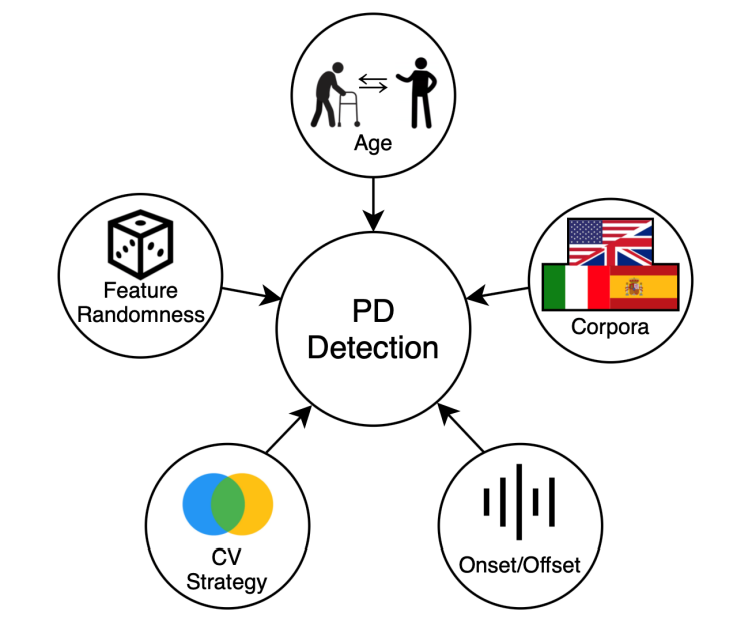
\includegraphics[width=0.4\textwidth]{./img/influence_of_factors_on_PD_detection}
	\caption{Czynniki powodujące zbyt optymistyczne wyniki detekcji PD na podstawie głosu \cite {SustainedVowelsProblems}}
    \label{fig:factors_PD_detection}
\end{figure}


\begin{enumerate}[label={\alph*)}]
	\item Pominięcie aspektu tożsamości mówcy przy konstruowaniu zbiorów treningowych i testowych
	\item[] W przypadku, gdy w zbiorze danych znajduje się kilka nagrań od tego samego mówcy, można postąpić na dwa sposoby.
Pierwszy z nich to podział według podmiotów (ang. \emph{subject-wise split}) polegający na tym, że nagrania od tej samej
osoby znajdują się albo w zbiorze treningowym, albo testowym, natomiast nigdy w obu na raz.
Drugie podejście to podział według rekordów (ang. \emph{record-wise split}), gdzie nagrania są losowo dzielone do zbiorów
lub intencjonalnie używa się nagrań od tej samej osoby zarówno w zbiorze testowym, jak i treningowym.
Okazuje się, że podejście typu \emph{record-wise} prowadzi do wyższej dokładności niż \emph{subject-wise split}, jeśli pozostałe założenia pozostają identyczne.
Prawdopodobnie wynika to z faktu, że klasyfikator nastawia się na wykrywanie unikalnych informacji indywidualnych,
reprezentowanych przez współczynniki takie jak MFCC, a nie rzeczywiste biomarkery lub wzorce PD\@.
Dlatego też rekomendowana jest technika \emph{subject-wise split}, aby uniknąć zbyt optymistycznych wyników.

  	\item Niezbalansowanie klas pod względem wieku
	\item[] W literaturze można znaleźć prace wykorzystujące zbiory danych, w których średni wiek mówców
w klasie osób chorych na PD różni się od średniego wieku w klasie osób zdrowych o ponad 5 lat.
Autorzy zapewniają o wysokiej skuteczności swoich rozwiązań, jednak pomijają informacje o ryzyku, że klasyfikator
uczy się wykrywać cechy powiązane z wiekiem, zamiast rzeczywistych wzorców PD\@.
Wyniki eksperymentów w publikacji~\cite{SustainedVowelsProblems} pokazują, że wraz ze wzrostem różnicy między średnim wiekiem uczestników z PD i HC,
dokładność klasyfikacji konsekwentnie rośnie (Rys.~\ref{fig:acc_and_age_diff}).
Na tej podstawie można stwierdzić, że związany z wiekiem wpływ na głos mówców może zaburzać wyniki otrzymywane przez klasyfikator.
Dlatego też zaleca się zbalansowanie używanych zbiorów danych, tak aby średnia różnica wieku między tymi dwoma klasami była jak najmniejsza.


\begin{figure}[htbp]
	\centering
	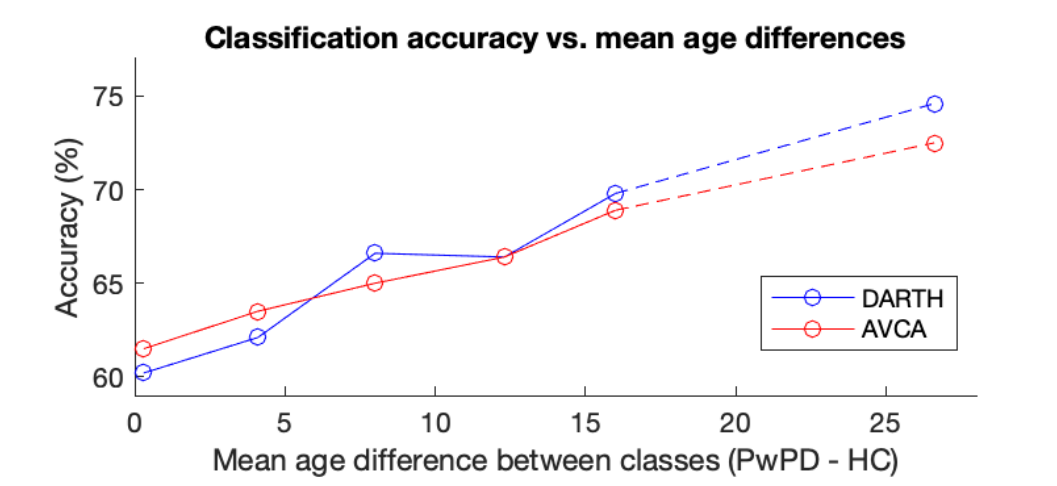
\includegraphics[width=0.7\textwidth]{./img/acc_and_age_difference}
	\caption{Wykres przedstawiający zależność różnicy wieku między klasami a dokładnością klasyfikacji~\cite {SustainedVowelsProblems}}
    \label{fig:acc_and_age_diff}
\end{figure}

  	\item wpływ losowości cech na dokładność klasyfikacji
	\item[] W publikacji~\cite{SustainedVowelsProblems} przeprowadzono badania analizujące wpływ losowości cech na dokładność klasyfikacji.
Zamieniono cechy obliczone za pomocą DARTH-VAT na losowe liczby, zachowując etykiety i podziały.
Wyniki wskazały, że nawet losowe cechy mogą prowadzić do wysokich wyników klasyfikacji (ponad 72\%).
Efekt ten jest bardziej widoczny w mniejszych korpusach, gdzie różnica między liczbą nagrań a wymiarowością cech ma większy wpływ na potencjalną korelację przypadkową.
Badanie pokazuje, że nadmierna liczba cech w stosunku do liczby obserwacji może prowadzić do fałszywie wysokich wyników klasyfikacji nawet przy użyciu losowych cech.
Im większa różnica między liczbą plików a wymiarem wektora cech, tym większe szanse na znalezienie cechy, która losowo koreluje z etykietami klas.
To sugeruje, że osiągnięcia klasyfikacyjne powinny być analizowane w kontekście proporcji cech do próbki, aby uniknąć nadmiernie optymistycznych interpretacji wyników klasyfikacji w zastosowaniach medycznych.

  	\item ograniczenie losowego nadmiernego dopasowania poprzez uwzględnienie zbioru walidacyjnego
	\item[] Dla mniejszych zbiorów danych, praktyką jest często używanie tylko zbiorów treningowych i testowych podczas krzyżowej walidacji.
Jest to podejście, które może prowadzić do wyników zbyt optymistycznych, ponieważ wszystkie wyniki testowe są brane pod uwagę przy wyborze optymalnej
konfiguracji modelu.
Inną strategią jest wykorzystanie danych treningowych do oceny wytrenowanych modeli i późniejsze przetestowanie najlepszego modelu na zbiorze testowym.
Niemniej jednak to podejście może być niepraktyczne, ponieważ może prowadzić do wyników idealnych (dokładność 100\%) na zbiorze treningowym, co jest niepożądane.
Aby uniknąć tych problemów, proponuje się wykorzystanie dodatkowego zbioru walidacyjnego~\cite{SustainedVowelsProblems}.
Wybierając model na podstawie wyników walidacyjnych, a następnie testując go na zbiorze testowym, można uniknąć ryzyka nadmiernego dopasowania.
Dla mniejszych zbiorów danych ta strategia może ograniczać dostępną liczbę danych treningowych, co wpływa na wydajność klasyfikacji.

	\item wpływ początku i końca  nagrań samogłosek na wyniki klasyfikacji
\item[] Główną różnicą między korpusami wykorzystywanymi do klasyfikacji choroby Parkinsona jest obecność fragmentów nagrania oznaczonych jako \emph{onset} i \emph{offset}.
Niektóre nagrania zawierają te segmenty, podczas gdy inne zostały ich pozbawione, aby zapewnić stabilniejszą fonację, co jest korzystne dla pewnych cech i algorytmów analizy.
W celu oceny znaczenia informacji zawartych w obszarach \emph{onset} i \emph{offset} dla klasyfikacji przeprowadzono eksperymenty porównawcze,
wykorzystując nagrania zarówno z fragmentami przyciętymi, jak i nieprzyciętymi~\cite{SustainedVowelsProblems}.
Wyniki tych eksperymentów ukazały, że wyeliminowanie fragmentów początkowych i końcowych wpłynęło negatywnie na dokładność klasyfikacji.
To wskazuje na to, że obszary te zawierają istotne informacje artykulacyjne, które mają znaczenie dla procesu klasyfikacji.

 	\item eksperymenty międzykorpusowe a zdolności generalizacyjne
	\item [] Większość badań dotyczących diagnozowania choroby Parkinsona na podstawie głosu opiera się na jednym lub ewentualnie kilku (wykorzystywanych niezależnie)
korpusach mowy.
W tym kontekście często pomija się badanie zdolności klasyfikatorów do ogólnego zastosowania.
W artykule~\cite{SustainedVowelsProblems} przeprowadzono międzykorpusowe eksperymenty na bazach danych w językach włoskim i hiszpańskim w celu
przetestowania zdolności ogólnych modeli.
Skuteczność tych modeli różniła się w zależności od języka zbioru testowego.
Może to wynikać z odmiennej różnorodności nagrań, co ma wpływ na stabilność modelu.
Drugim możliwym wyjaśnieniem jest to, że głos osób z chorobą Parkinsona może być w różnym stopniu obarczony objawami choroby w zależności od języka ojczystego lub stopnia zaawansowania choroby.
Innymi słowy, w zależności od użytego zbioru danych objawy mogą być nasilone w różny sposób i konieczne jest wzięcie tego pod uwagę tak by zdolności generalizacyjne modelu były jak najwyższe.
\end{enumerate}


Identyfikacja i świadomość wpływu powyższych czynników pozwala na dostosowaniu przeprowadzanych eksperymentów tak, aby uniknąć wyników zbyt optymistycznych.
Usystematyzowanie podejścia do analizy głosu pod kątem diagnostyki choroby Parkinsona przyczyni się do możliwości obiektywnego porównania istniejących i nowych rozwiązań.
Tym samym przyspieszy to postęp w tej dziedzinie i uzyskanie optymalnego rozwiązania, które mogłoby zostać wykorzystane w rzeczywistym środowisku.

Nie są to jednak wszystkie czynniki, które zaburzają obiektywność wyników.
Konieczna jest dyskusja na temat nowych kompleksowych linii bazowych dla prowadzenia eksperymentów w automatycznym wykrywaniu PD na podstawie fonacji,
a także innych ogólnych zastosowań przetwarzania mowy.

Prace nad automatyczną detekcją Parkinsona na podstawie głosu trwają już od dłuższego czasu.
Jednak wciąż brakuje systemu, który mógłby zostać uznany za wystarczająco niezawodne narzędzie diagnostyczne.
Wśród problemów, które ograniczają rzeczywiste wykorzystanie takich systemów wyróżnia się:
\begin{itemize}[itemsep=0.1pt]
	\item zróżnicowanie wzorców mowy: osoby z chorobą Parkinsona mogą różnić się w sposób, w jaki zmiany w mowie wpływają na ich głos.
To zróżnicowanie utrudnia stworzenie uniwersalnego modelu, który działałby skutecznie dla wszystkich pacjentów.
	\item wpływ zmiennych czynników: wpływ na mowę mogą mieć różne czynniki, takie jak zmęczenie, stres czy otoczenie akustyczne.
Te zmienne mogą wprowadzać zakłócenia w analizie mowy i utrudniać jednoznaczną diagnozę.
	\item potrzeba dużej bazy danych: aby stworzyć dokładny system detekcji, konieczne jest posiadanie dużej bazy danych głosów osób z i
bez choroby Parkinsona.
Uzyskanie takiej bazy danych, która odzwierciedla różnorodność pacjentów i warunki środowiskowe, może być wyzwaniem.
Większość publikacji opiera się na bazach danych zawierających około 50 nagrań, co nie jest wystarczająco reprezentatywną próbą.
	\item wczesne wykrycie i subtelne objawy: wczesne stadia choroby Parkinsona często manifestują się subtelnie, a różnice w mowie mogą być
trudne do zauważenia.
To może prowadzić do błędnych diagnoz lub niskiej skuteczności systemu.
	\item weryfikacja i walidacja: Aby narzędzie diagnostyczne oparte na mowie było skuteczne, musi być poddane rygorystycznym testom w rzeczywistych
warunkach klinicznych.
Weryfikacja i walidacja takiego systemu to skomplikowany proces.
	\item ograniczenia technologiczne: pomimo postępów w technologii analizy mowy, istnieją nadal ograniczenia w dokładności i precyzji takich systemów.
Może to prowadzić do wyników fałszywie pozytywnych lub negatywnych.
	\item aspekty etyczne i prywatność: wykorzystywanie danych głosowych do diagnozowania chorób podnosi kwestie związane z prywatnością i etyką.
Konieczne jest zagwarantowanie odpowiednich zabezpieczeń danych i zgody pacjentów na wykorzystanie ich informacji w celach medycznych.
\end{itemize}

Mimo tych wyzwań, prace nad wykorzystaniem analizy mowy do diagnozowania choroby Parkinsona są obiecujące i mogą przyczynić się do poprawy jakości życia
pacjentów oraz usprawnienia procesu diagnozy i leczenia.
Jednakże przed stworzeniem skutecznego narzędzia diagnostycznego opartego na głosie jest jeszcze wiele pracy do wykonania

W niniejszej pracy podjęta zostanie próba implementacji takiego rozwiązania.
Uwzględnione zostaną wszystkie z rekomendacji przedstawionych w artykule~\cite{SustainedVowelsProblems}.
\chapter{Materiał i metoda badawcza\@}
\label{ch:material-badawczy}

Przegląd literatury ukazuje obfitość raportów dotyczących identyfikacji choroby Parkinsona na podstawie krótkich fragmentów mowy, takich jak samogłoski, sylaby, czy krótkie słowa i zdania.
W tych badaniach wykorzystywane są różnorodne zadania wokalne, metody ekstrakcji cech oraz klasyfikacji.
Jednak wiele czynników wpływa na trudność obiektywnego porównania proponowanych rozwiązań, w tym różnice w wykorzystywanych bazach danych.

W niniejszej pracy przeprowadzono porównanie skuteczności wybranych architektur sieci konwolucyjnych oraz ocenić ich przydatność w diagnozowaniu choroby Parkinsona na podstawie różnych samogłosek.
Zastosowano  połączenie trzech różnych baz danych w celu poszerzenia zbioru o dodatkowe wzorce.

W tym rozdziale przedstawiono szczegółowy opis danych użytych do porównania efektywności i wydajności różnych algorytmów w diagnozowaniu choroby Parkinsona na podstawie mowy.
Omówiono proces przygotowania sygnałów oraz parametryzację sygnału akustycznego.
Następnie przedstawiono opis algorytmów, które zostały wykorzystane do realizacji postawionych zadań.
Schemat przyjętego podejścia został zilustrowany na Rys.~\ref{fig:methodology}.


\begin{figure}[htbp]
	\centering
	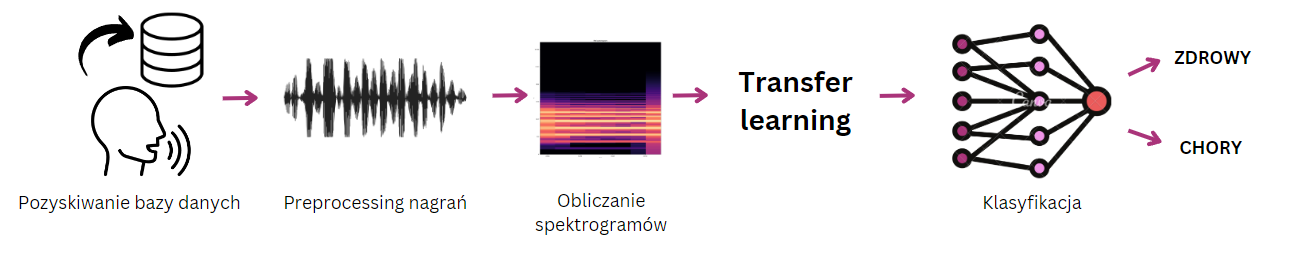
\includegraphics[width=1\textwidth]{./img/methodology}
	\caption{Schemat przyjętego podejścia\@}
    \label{fig:methodology}
\end{figure}

%---------------------------------------------------------------------------

\section{Materiał badawczy}
\label{sec:material-badawczy}

Materiałem badawczym w niniejszej pracy magisterskiej są nagrania głosowe podtrzymywanych samogłosek (ang. \emph{sustained vowels}) /a/, /e/, /i/, /o/ oraz /u/.
Baza danych obejmuje nagrania osób zdrowych oraz cierpiących na chorobę Parkinsona.
Podstawą skuteczności metod uczenia maszynowego jest odpowiednie przygotowanie danych, zarówno pod względem jakości, jak i ilości.
To kluczowy element, który wpływa na wydajność i zdolność modelu do radzenia sobie w rzeczywistym środowisku.
Dane użyte do trenowania modelu muszą być dokładne, spójne i reprezentatywne dla rzeczywistego środowiska, w którym będzie działał model.
Jest to podobne do procesu nauki lekarza – im więcej przypadków lekarz widzi i diagnozuje, tym lepiej radzi sobie z różnymi przypadkami w praktyce.
W  uczeniu maszynowym większa ilość danych pozwala na uchwycenie różnic międzyosobniczych i niuansów w danych, co przekłada się na większą stabilność i skuteczność modelu.
Model musi być w stanie radzić sobie z nowymi danymi, które nie były używane podczas treningu.

W pracy wykorzystano dane, zarejestrowane dla 3 różnych języków: polskiego, włoskiego oraz hiszpańskiego.
Wykorzystanie baz danych uwzględniając różne grupy językowe pozwala na analizę uniwersalności narzędzia służącego do automatycznej diagnozy choroby Parkinsona, tak by nie było ono ograniczone tylko do jednej grupy narodowościowej czy geograficznej.
Takie podejście pozwala na utworzenie modelu uniwersalnego, który mógłby być używany na skalę międzynarodową przyczyniając się do poprawy jakości opieki zdrowotnej i diagnozy tej choroby.

Warto też zauważyć, że żadna z dostępnych publicznie baz danych nie zawiera wystarczającej ilości nagrań, by mówić o stabilnym rozwiązaniu, które mogłoby zostać użyte na szeroką skalę.
Łączenie zestawów danych może znacząco poprawić zdolności generalizacyjne modelu.

\subsection{Baza danych w języku polskim}
\label{subsec:polska-baza}

Materiał badawczy pochodzący od osób cierpiących na chorobę Parkinsona (PD) i posługujących się językiem polskim, został zgromadzony w ramach
realizacji rozprawy doktorskiej we współpracy z Krakowskim Szpitalem Specjalistycznym im.
Jana Pawła II~\cite{daria:2018}.
W bazie danych znajdują się nagrania samogłosek /a/, /e/, /i/, /o/ oraz /u/ z wydłużoną intonacją, pozyskane od 27 pacjentów.
Dla każdego z pacjentów dostępne jest jedno nagranie każdej z wymienionych samogłosek.
W ramach przeprowadzonych badań pomiary zostały wykonane przed spożyciem leków oraz w określonych odstępach czasowych po podaniu lewodopy.
Przed każdym pomiarem lekarz neurolog przeprowadzał badanie pacjenta i oceniał jego stan, wykorzystując skalę UPDRS\@.
W niniejszej pracy magisterskiej wykorzystano jedynie nagrania głosowe zarejestrowane przed podaniem leku.

Nagrania osób zdrowych zostały zebrane w ramach tej pracy magisterskiej przy wykorzystaniu aplikacji \emph{Easy Voice Recorder}.
Ustalono protokół nagrywania, wykluczając osoby poniżej 50 roku życia, palące oraz ze zdiagnozowaną lub podejrzewaną chorobą wpływającą na aparat mowy, lub korę mózgową (np.
choroba Parkinsona, epilepsja, padaczka).
Pozyskiwano nagrania jedynie od osób, dla których językiem ojczystym jest polski.
Każda osoba kwalifikująca się do badania otrzymała zadanie trzykrotnego wypowiedzenia samogłosek /a/, /e/, /i/, /o/ oraz /u/ w odstępach czasowych, utrzymując dźwięk przez co najmniej 2 sekundy.
Następnie nagrania zostały dokładnie przeanalizowane.
Usunięto nagrania zbyt krótkie oraz te, które nie spełniały kryteriów dotyczących jakości.
Otrzymana baza danych nadal zawierała nagrania od 27 osób chorych oraz od 26 osób zdrowych, zmieniła się jedynie liczebność nagrań dla poszczególnych samogłosek.
W tabeli~\ref{tab:polish_database} przedstawiono informacje dotyczące bazy danych.

\begin{table}[h]
\centering
\caption{Charakterystyka polskiej bazy danych}
\label{tab:polish_database}
\begin{tabular}{|l|c|c|c|}
\hline
\textbf{Kategoria} &\textbf{Osoby zdrowe (HC)} &\textbf{Osoby chore (PD)} &\textbf{Razem} \\ \hline
Liczba osób &26 &27 &53\\ \hline
Liczba nagrań &67 &27 &94\\ \hline
Średnia wieku &60,88 ± 7,98 &64,49 ± 8,49  &62,68 ± 8,43\\ \hline
Liczba kobiet &18 &13 &31\\ \hline
Liczba mężczyzn &8 &14 &22 \\ \hline
\end{tabular}
\end{table}

\subsection{Baza danych w języku włoskim}
\label{subsec:wloska-baza}

Włoska baza danych to \emph{Italian Parkinson's Voice And Speech}, która dostępna jest na platformie \emph{IEEEDataPort}~\cite{italian-database}.
Zbiór zawiera wiele różnych podzbiorów, ale wykorzystano jedynie podtrzymywane samogłoski /a/, /e/, /i/, /o/ oraz /u/.
Ocena stopnia zaawansowania choroby została przeprowadzona przy pomocy skali UPDRS\@.
Wszystkie nagrania pochodzą od osób, dla których natywnym językiem jest włoski.
Początkowo baza danych zawiera nagrania od 50 osób, jednak po wstępnym oczyszczeniu wykorzystano jedynie 45.
Charakterystykę zbioru przedstawiono w tabeli~\ref{tab:italian-database}

\begin{table}[h]
\centering
\caption{Charakterystyka włoskiej bazy danych}
\label{tab:italian-database}
\begin{tabular}{|l|c|c|c|}
\hline
\textbf{Kategoria} &\textbf{Osoby zdrowe (HC)} &\textbf{Osoby chore (PD)} &\textbf{Razem} \\ \hline
Liczba osób &19 &26 &45\\ \hline
Liczba nagrań &38 &52 &90\\ \hline
Średnia wieku &67,31 ± 5,23 &66,96 ± 8,59  & 67,11 ± 7,36 \\ \hline
Liczba kobiet &10 &7 &17\\ \hline
Liczba mężczyzn &9 &19 &28 \\ \hline
\end{tabular}
\end{table}


\subsection{Baza danych w języku hiszpańskim}
\label{subsec:hiszpanska-baza}


Hiszpańska baza danych (PC-GITA) ~\cite{pc-gita} zawiera nagrania mowy 50 pacjentów z PD i tyle samo osób zdrowych, dopasowanych pod względem wieku i płci.
Wszyscy uczestnicy posługują się kolumbijską odmianą języka hiszpańskiego, a nagrania zostały zebrane zgodnie z protokołem uwzględniającym wymagania techniczne oraz zalecenia ekspertów z dziedzin lingwistyki, foniatrii i neurologii.
Kolekcja obejmuje takie zadania jak podtrzymywane wymawianie samogłosek, ocenę diadokokinetyczną, 45 słów, 10 zdań, tekst do czytania i monolog.
Podobnie jak w przypadku pozostałych baz wykorzystano jedynie nagrania samogłosek /a/, /e/, /i/, /o/ oraz /u/.
Na jednego uczestnika przypadają trzy powtórzenia każdej z samogłosek.
Szczegółowa charakterystyka zbioru została przedstawiona w tabeli~\ref{tab:spanish-database}

\begin{table}[ht]
\centering
\caption{Charakterystyka hiszpańskiej bazy danych}
\label{tab:spanish-database}
\begin{tabular}{|l|c|c|c|}
\hline
\textbf{Kategoria} &\textbf{Osoby zdrowe (HC)} &\textbf{Osoby chore (PD)} &\textbf{Razem} \\ \hline
Liczba osób &50 &50 &100\\ \hline
Liczba nagrań &150 &150 &300\\ \hline
Średnia wieku &60,90 ± 9,37 &61,14 ± 9,51  &61,02 ± 9,15\\ \hline
Liczba kobiet &25 &25 &50\\ \hline
Liczba mężczyzn &25 &25 &50 \\ \hline
\end{tabular}
\end{table}

\section*{}
Połączenie baz danych było możliwe ze względu na uniwersalność podstawy diagnostycznej, jaką są podtrzymywane samogłoski.
Nagrania różniły się długością, jednak wykorzystano jedynie krótkie fragmenty (0,1 s), więc nie stanowiło to problemu.
Wszystkie zostały zarejestrowane z częstotliwością próbkowania 44,1 kHz.

Trudno nie zauważyć znaczącej przewagi liczby nagrań w bazie hiszpańskojęzycznej (Rys.~\ref{fig:language-distribution}).
Jednak zrezygnowano z wyrównywania liczby nagrań w poszczególnych językach, z uwagi na to, że baza danych jest już stosunkowo niewielka, i dodatkowe ograniczenie liczby nagrań mogłoby znacząco zmniejszyć jej wartość i możliwości badawcze.
Zachowano zbliżone proporcje wieku (różnica w średniej wieku mniejsza niż 5 lat) i płci pomiędzy grupą pacjentów a grupą porównawczą.
Drobne różnice w liczbie próbek w poszczególnych przedziałach wiekowych nie powinny mieć istotnego wpływu na wyniki klasyfikacji.
Liczba nagrań dla każdej samogłoski została wyrównana, tak by umożliwić obiektywne porównanie ich potencjalnego wykorzystania.
Szczegółowe charakterystyki zbioru danych zostały przedstawione na Rys.~\ref{fig:charakterystyka-bazy}.


\begin{figure}
    \begin{subfigure}{0.9\textwidth}
        \centering
       	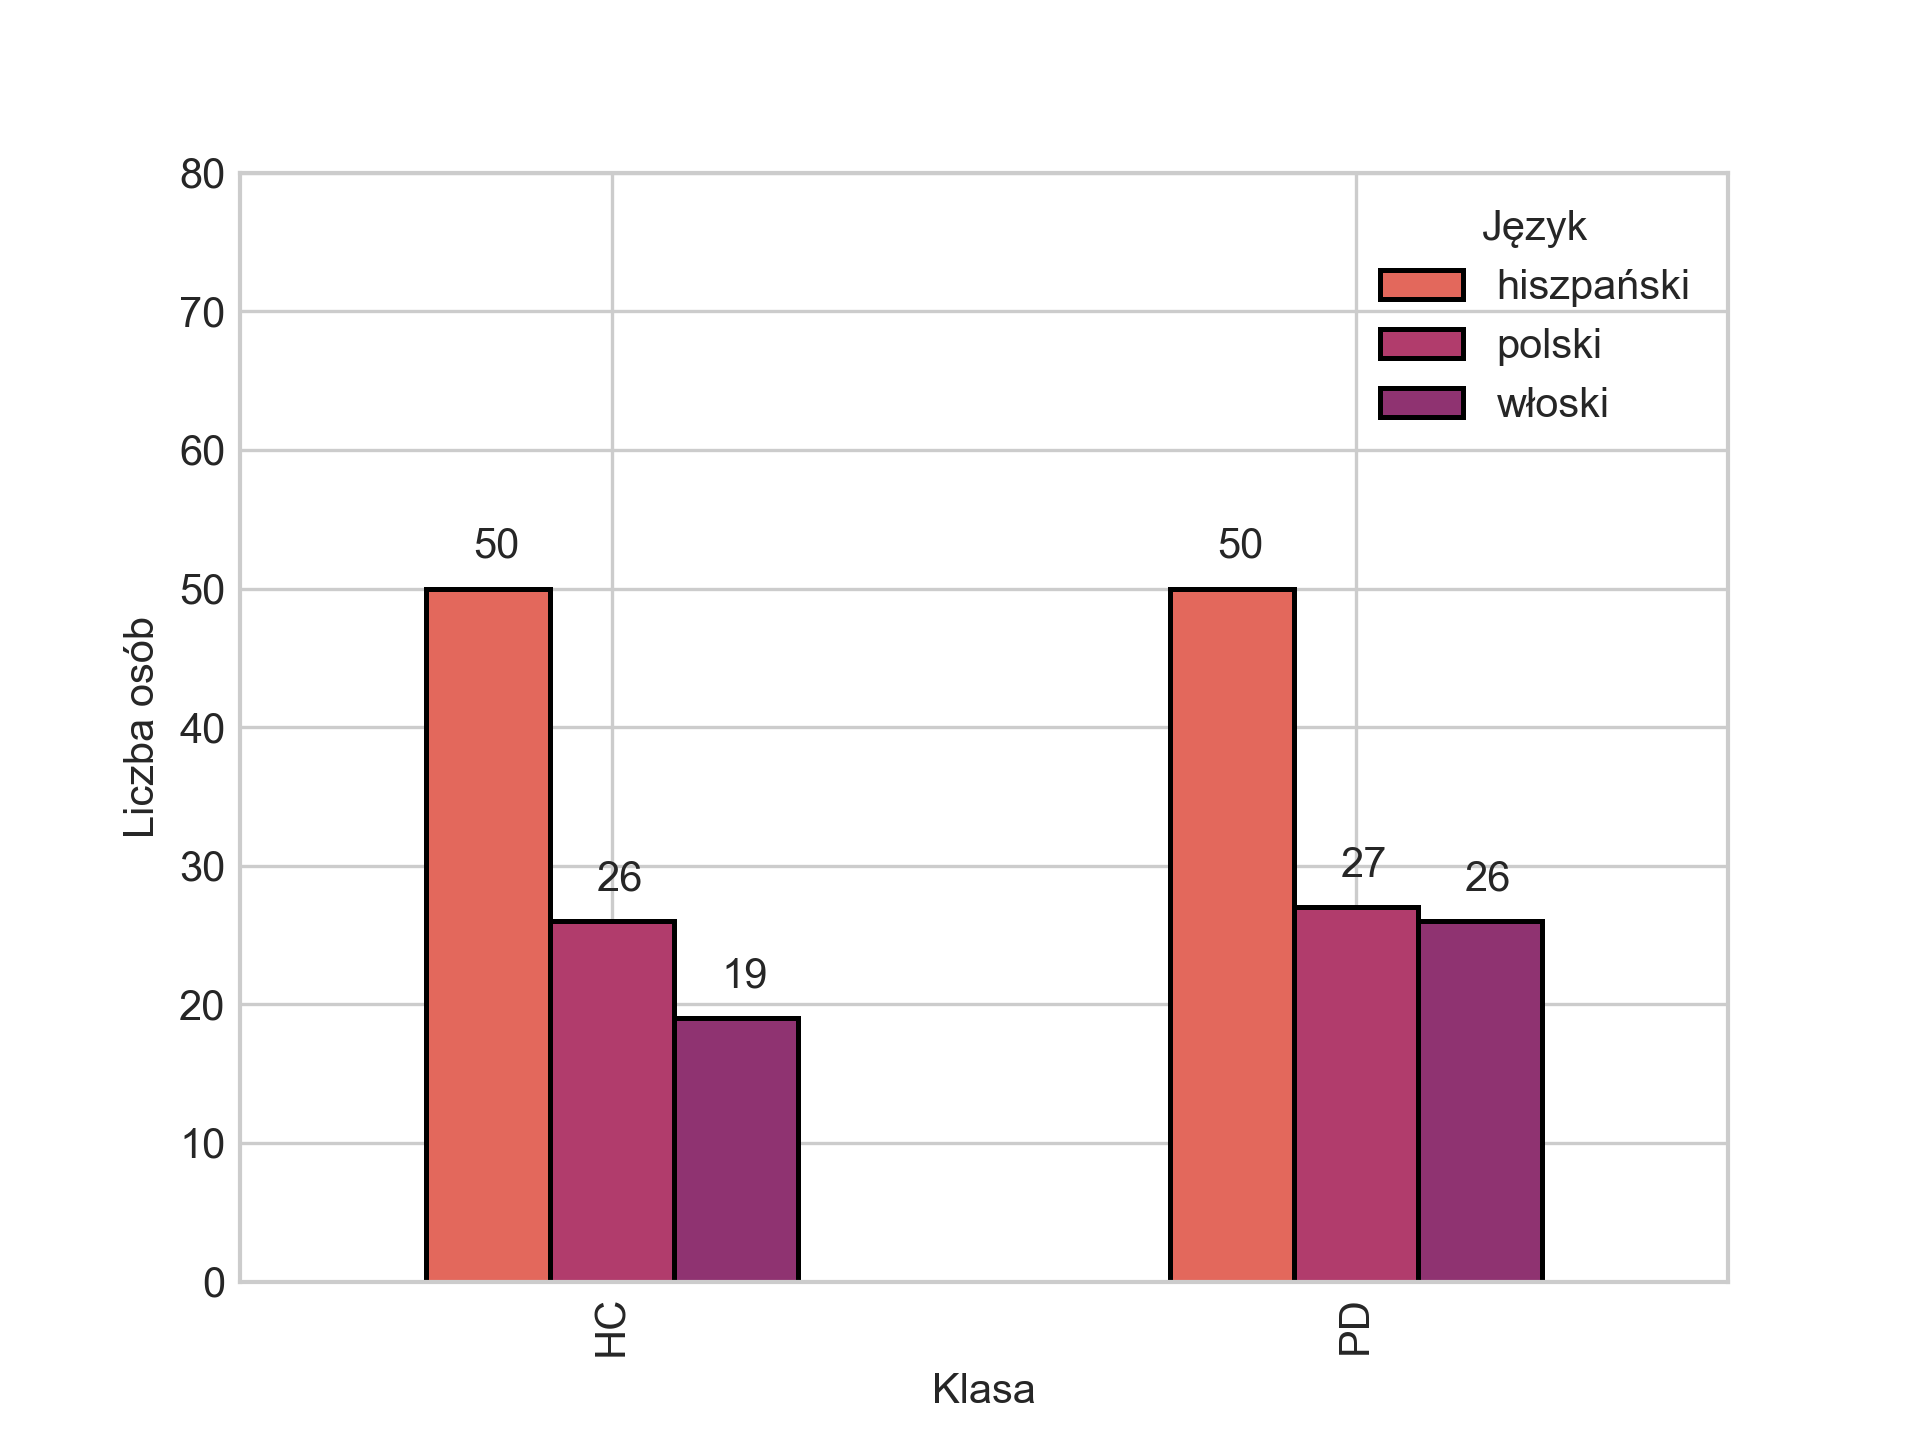
\includegraphics[width=0.60\textwidth]{./img/database stats/languages_distribution}
	    \caption{Udział nagrań z poszczególnych grup językowych}
        \label{fig:language-distribution}
    \end{subfigure}

    \begin{subfigure}{0.85\textwidth}
        \centering
        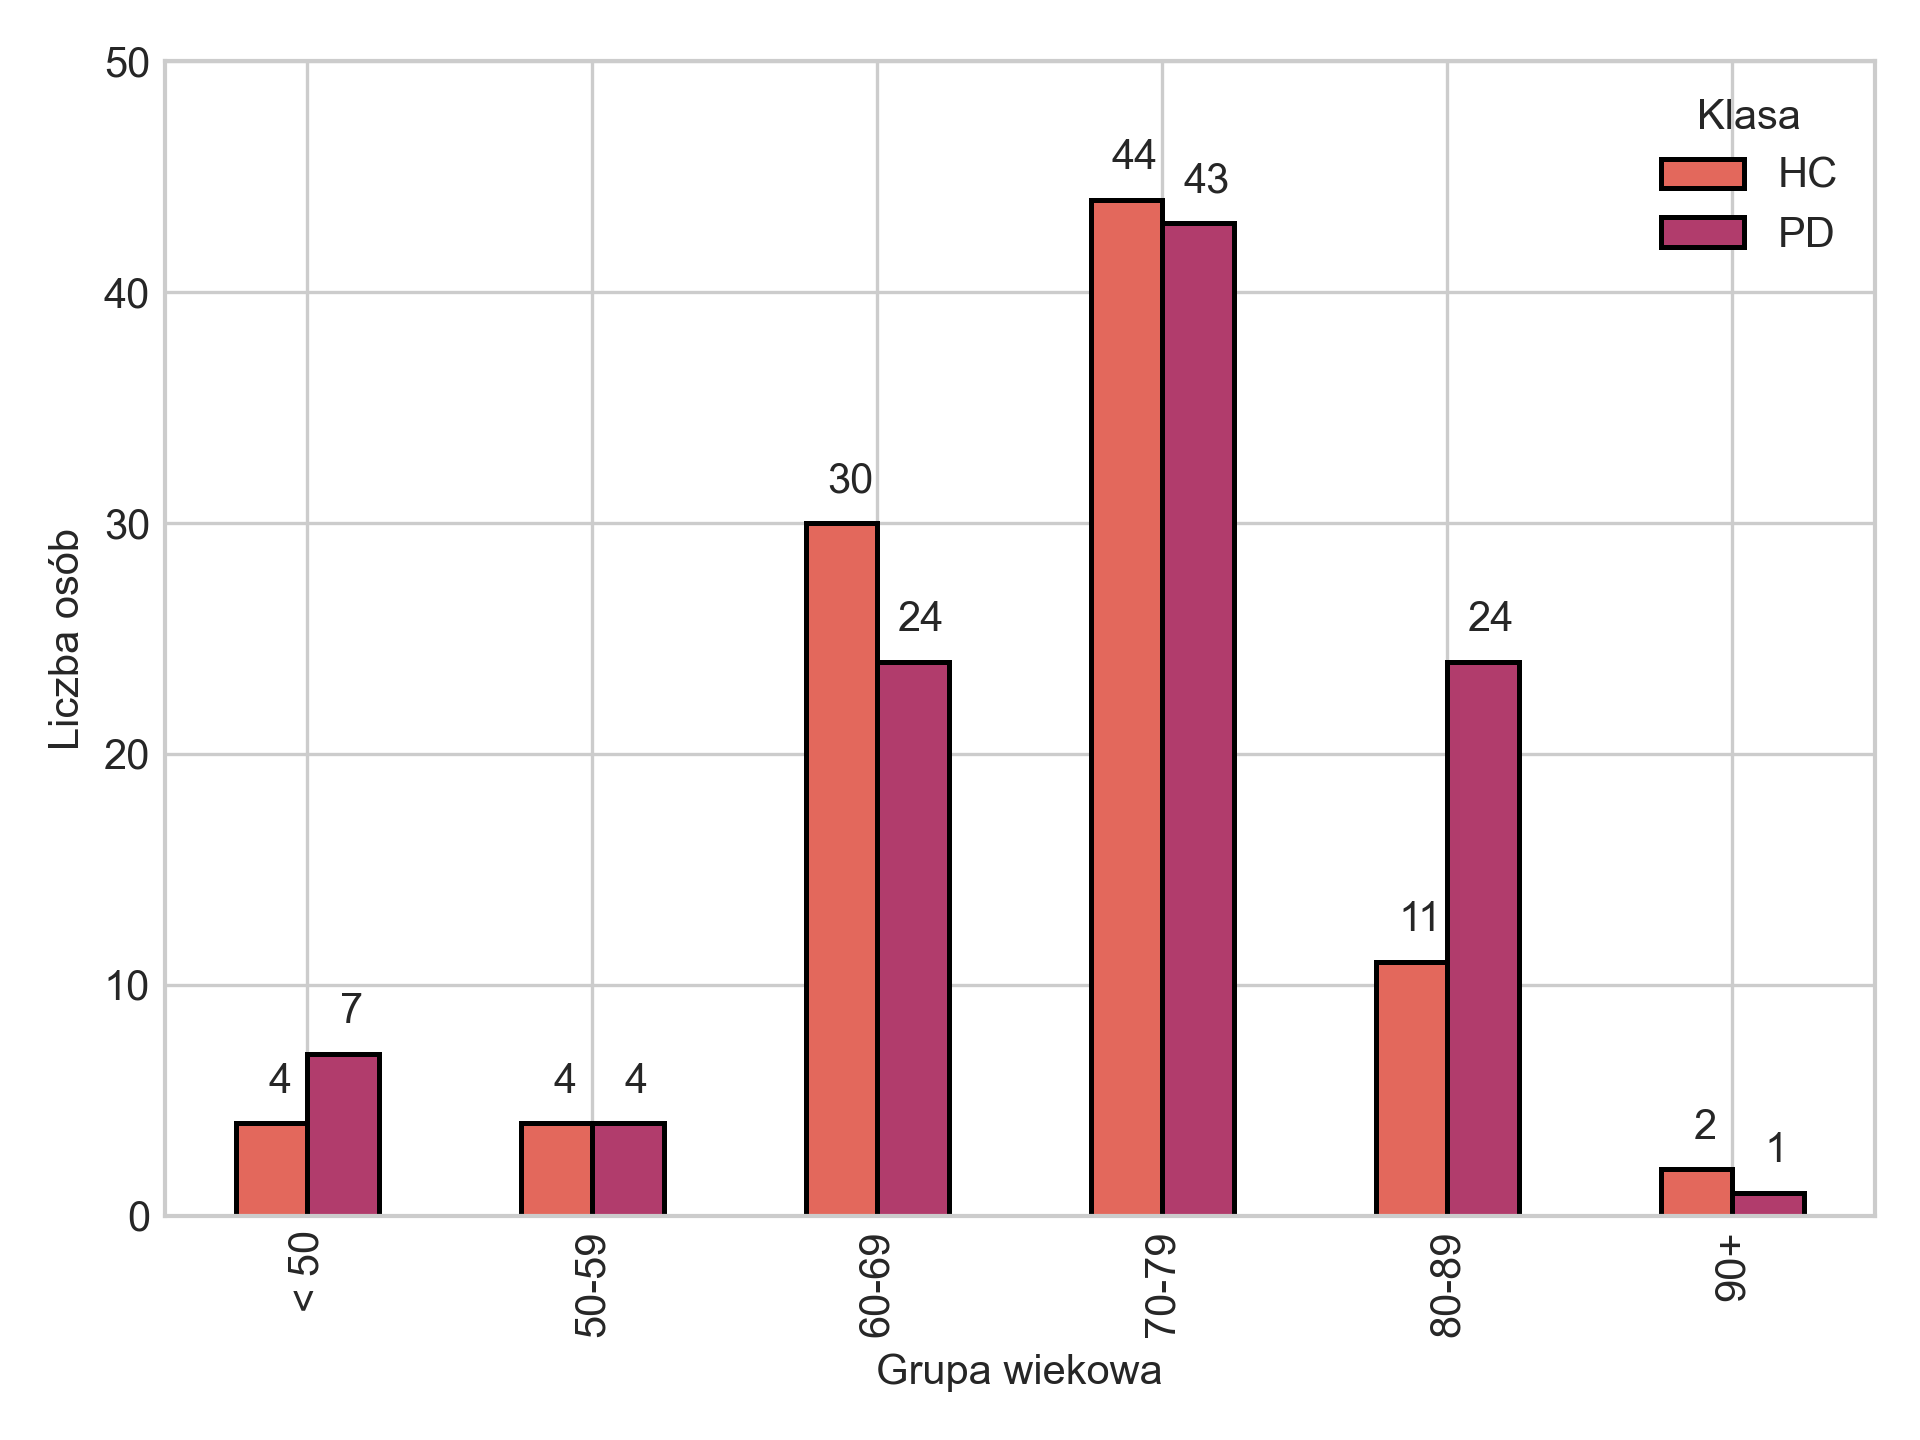
\includegraphics[width=0.60\textwidth]{./img/database stats/age_distribution}
        \caption{Rozkład grup wiekowych w poszczególnych klasach}
        \label{fig:age-distribution}
    \end{subfigure}

    \begin{subfigure}{0.85\textwidth}
        \centering
       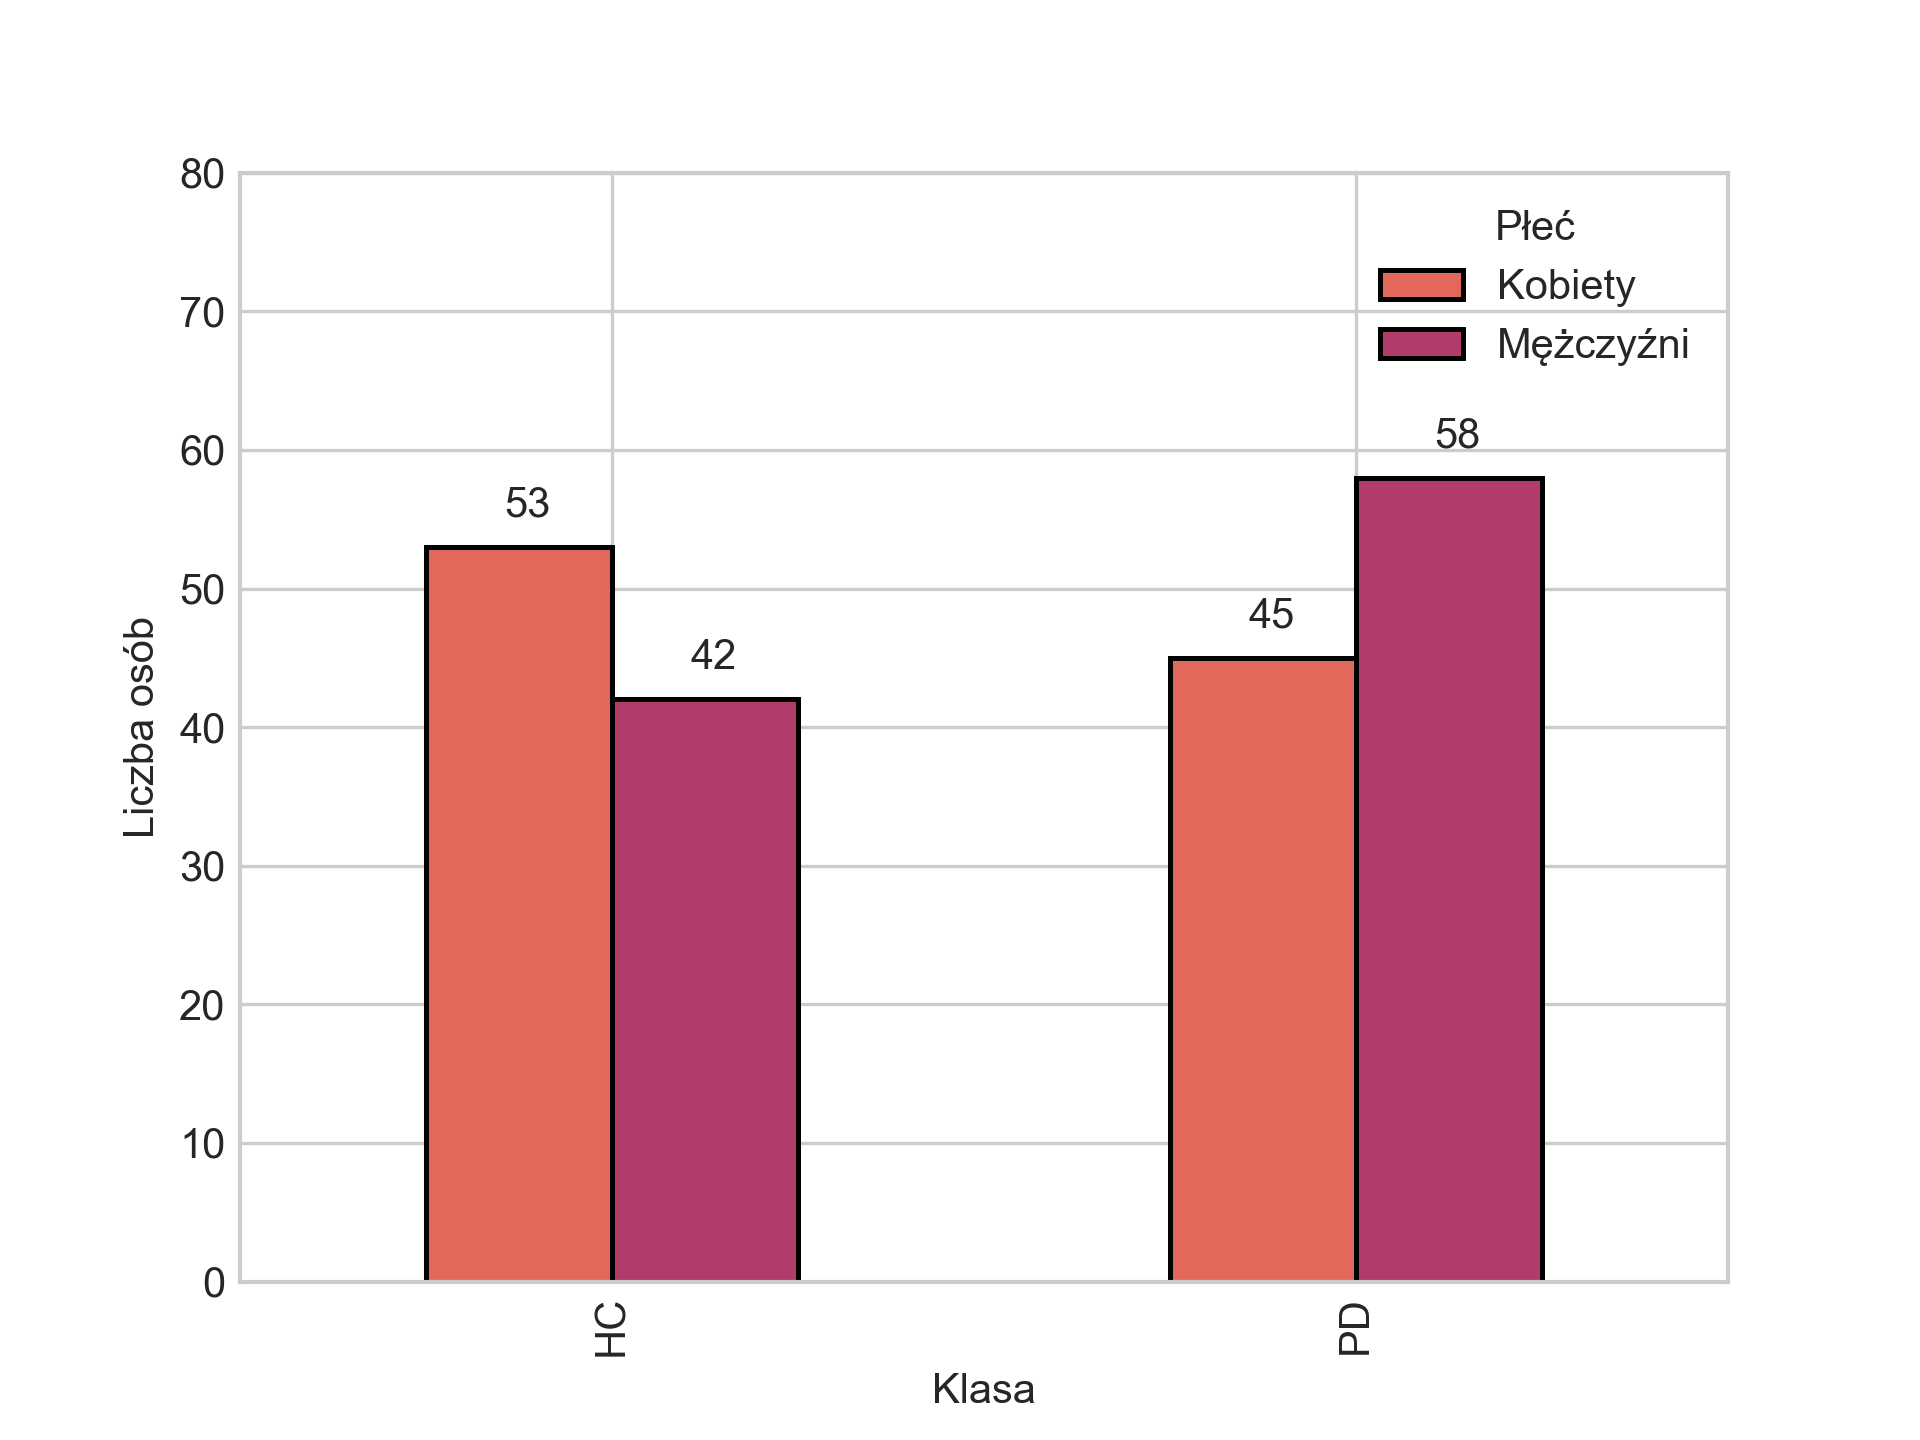
\includegraphics[width=0.65\textwidth]{./img/database stats/gender_distribution}
	    \caption{Rozkład płci w klasach}
        \label{fig:gender-distribution}
    \end{subfigure}

    \caption{Charakterystyka wykorzystanej bazy danych. (a) stosunek liczby osób z poszczególnych grup językowych;
        (b) rozkład wiekowy w grupie osób z chorobą Parkinsona i grupie osób zdrowych; (c) rozkład płci w grupie osób z PD i grupie osób zdrowych.}
    \label{fig:charakterystyka-bazy}
\end{figure}



\begin{table}[h]
\centering
\caption{Charakterystyka stworzonej bazy danych}
\label{tab:summary-database}
\begin{tabular}{|l|c|c|c|}
\hline
\textbf{Kategoria} &\textbf{Osoby zdrowe (HC)} &\textbf{Osoby chore (PD)} &\textbf{Razem} \\ \hline
Liczba osób &95 &103 &198\\ \hline
Liczba nagrań &255 &229 &484\\ \hline
Średnia wieku & 62,18 ± 8,70 & 62,84 ± 9,45  & 62,32 ± 8,99 \\ \hline
Liczba kobiet &53 &45 &98\\ \hline
Liczba mężczyzn &42 &58 &100 \\ \hline
\end{tabular}
\end{table}
%---------------------------------------------------------------------------

\section{Parametryzacja sygnału akustycznego}
\label{sec:parametryzacja-sygnalu-akustycznego}

W kontekście projektowania rozwiązań związanych z uczeniem maszynowym, jednym z kluczowych aspektów jest staranne przygotowanie danych.
Proces ten jest niezwykle istotny i obejmuje kilka kluczowych etapów, które mają ogromny wpływ na jakość i skuteczność modelu.
Dwa główne etapy, które wymagają szczególnej uwagi, to preprocessing i ekstrakcja cech.
Preprocessing odnosi się do przetwarzania wstępnego danych dźwiękowych przed ich podaniem modelowi uczenia maszynowego.
W ramach tego procesu usuwane są zakłócenia, szumy i niepożądane.
W przypadku nagrań może to obejmować filtrację, normalizację głośności, usuwanie niepotrzebnych fragmentów dźwięku oraz inne techniki poprawiające jakość sygnału.
Poprawne wykonanie etapu preprocessingu może znacząco wpłynąć na  jakość wyników uzyskiwanych przez modele.
Drugim istotnym etapem jest ekstrakcja cech.
W ramach tego procesu z nagrań mowy wydobywane są istotne parametry lub cechy, które mogą być używane przez modele uczenia maszynowego do rozpoznawania wzorców.
Wybór odpowiednich cech i ich dokładna ekstrakcja mają kluczowe znaczenie, ponieważ to od nich zależy, jakie informacje zostaną dostarczone modelowi do analizy.

\subsection{Przygotowanie nagrań}
\label{subsec:preprocessing}

Nagrania zostały przycięte, tak by nie zawierały początkowych i końcowych fragmentów ciszy.
Ten proces eliminuje niepotrzebne fragmenty i skupia analizę jedynie na istotnych fragmentach mowy, co może poprawić skuteczność modelu.
W celu automatycznego usunięcia niepożądanych fragmentów skorzystano z pakietu \emph{Librosa} do, a następnie każde z nagrań zostało przeanalizowane w programie \emph{Audacity}.
Upewniono się, że nagrania zostały poprawnie przetworzone oraz wprowadzono ręcznie ewentualne poprawki.

Z uwagi na wykorzystanie różnych baz danych, charakteryzujących się zróżnicowanymi warunkami nagrywania, zdecydowano się na ograniczenie wpływu otoczenia na dokładność klasyfikacji.
W tym celu zastosowano filtr pasmowoprzepustowy, który pozwolił na eliminację niepotrzebnych częstotliwości, które mogą nie mieć znaczenia dla analizy mowy.
Wykorzystanie tego filtru zapobiegło również jedynie dostosowaniu modelu do cech charakteryzujących odstające częstotliwości, takie jak chrypka czy inne zakłócenia dźwiękowe.
W efekcie przekazywane były jedynie częstotliwości zawarte w przedziale między 500 Hz a 1500 Hz.

Wykorzystano bardzo krótkie fragmenty nagrań o długości 0,1 s.
Sygnały po przekształceniach przedstawiono na rysunku~\ref{fig:recordings}.

\begin{figure}[ht]
    \centering
    \begin{subfigure}{0.49\textwidth}
        \centering
        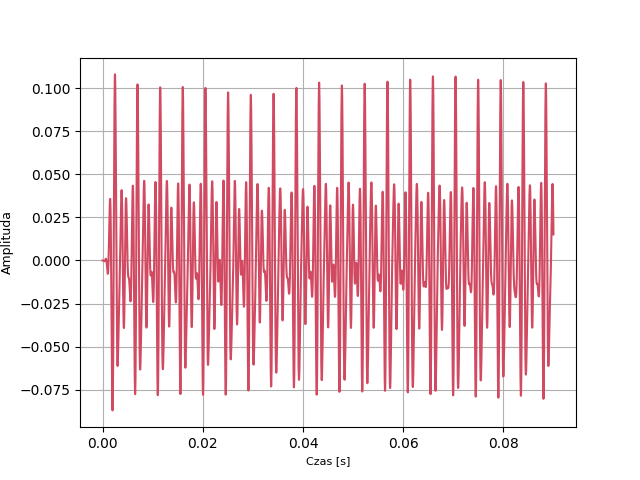
\includegraphics[width=\textwidth]{./img/recordings/HC_a}
        \caption{Sygnał głosu osoby zdrowej (HC)\@}
        \label{fig:recording_HC}
    \end{subfigure}
    \begin{subfigure}{0.49\textwidth}
        \centering
        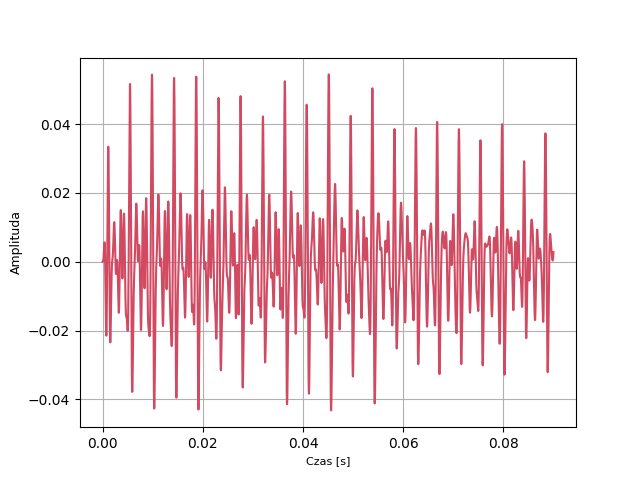
\includegraphics[width=\textwidth]{./img/recordings/PD_a}
        \caption{Sygnał głosu osoby z PD\@}
        \label{fig:recording_PD}
    \end{subfigure}

    \caption{Przykładowe nagrania samogłoski /a/ po preprocessingu (a) dla osoby zdrowej oraz (b) dla osoby z chorobą Parkinsona.}
    \label{fig:recordings}
\end{figure}

\subsection{Obliczanie mel-spektrogramów}
\label{subsec:melspectrogram}

Zdecydowano się na przedstawienie przygotowanych nagrań w formie graficznej w postaci mel-spektrogramów, które zostaną następnie użyte do dalszej analizy.
Spektrogramy to graficzna reprezentacja zmian widma dźwięku w funkcji czasu.
Wykorzystując transformację Fouriera, sygnał dźwiękowy jest podzielony na krótkie ramki czasowe, a następnie dla każdej ramki obliczane jest widmo amplitudowe.
Spektrogram przedstawia te widma w formie kolorowej mapy, gdzie oś pozioma reprezentuje czas, oś pionowa reprezentuje częstotliwość, a intensywność koloru oznacza amplitudę.
Spektrogramy są często wykorzystywane w analizie dźwięku i sygnałów akustycznych.
Pozwalają one zobaczyć, jak zmienia się struktura częstotliwościowa dźwięku w czasie, co może być przydatne do analizy cech akustycznych, identyfikacji dźwięków, diagnostyki medycznej czy rozpoznawania mowy.
Dzięki spektrogramom można wizualnie analizować zmiany w widmie dźwięku, takie jak formanty samogłoskowe, obecność szumów czy artefaktów.

Natomiast mel-spektrogramy to wariant spektrogramów, w których oś częstotliwości jest przekształcona na skalę Mel, czyli nieliniową skalę częstotliwości, która bardziej odpowiada percepcji ludzkiego słuchu.
Stosuje się ją, aby lepiej odzwierciedlić sposób, w jaki odbieramy i rozpoznajemy różnice między różnymi tonami dźwięków.
Przez uwzględnienie charakterystyk percepcji słuchowej człowieka, mel-spektrogramy dostarczają bardziej reprezentatywnych danych akustycznych dla analizy i klasyfikacji dźwięku.
Proces obliczeń mel-spektrogramów został zrealizowany przy użyciu biblioteki języka Python, Librosa.
Wygenerowane mel-spektrogramy zostały przedstawione jako obrazy w skali logarytmicznej (Rys.~\ref{fig:melspectrograms}).

\begin{figure}[ht]
    \centering
    \begin{subfigure}{0.49\textwidth}
        \centering
        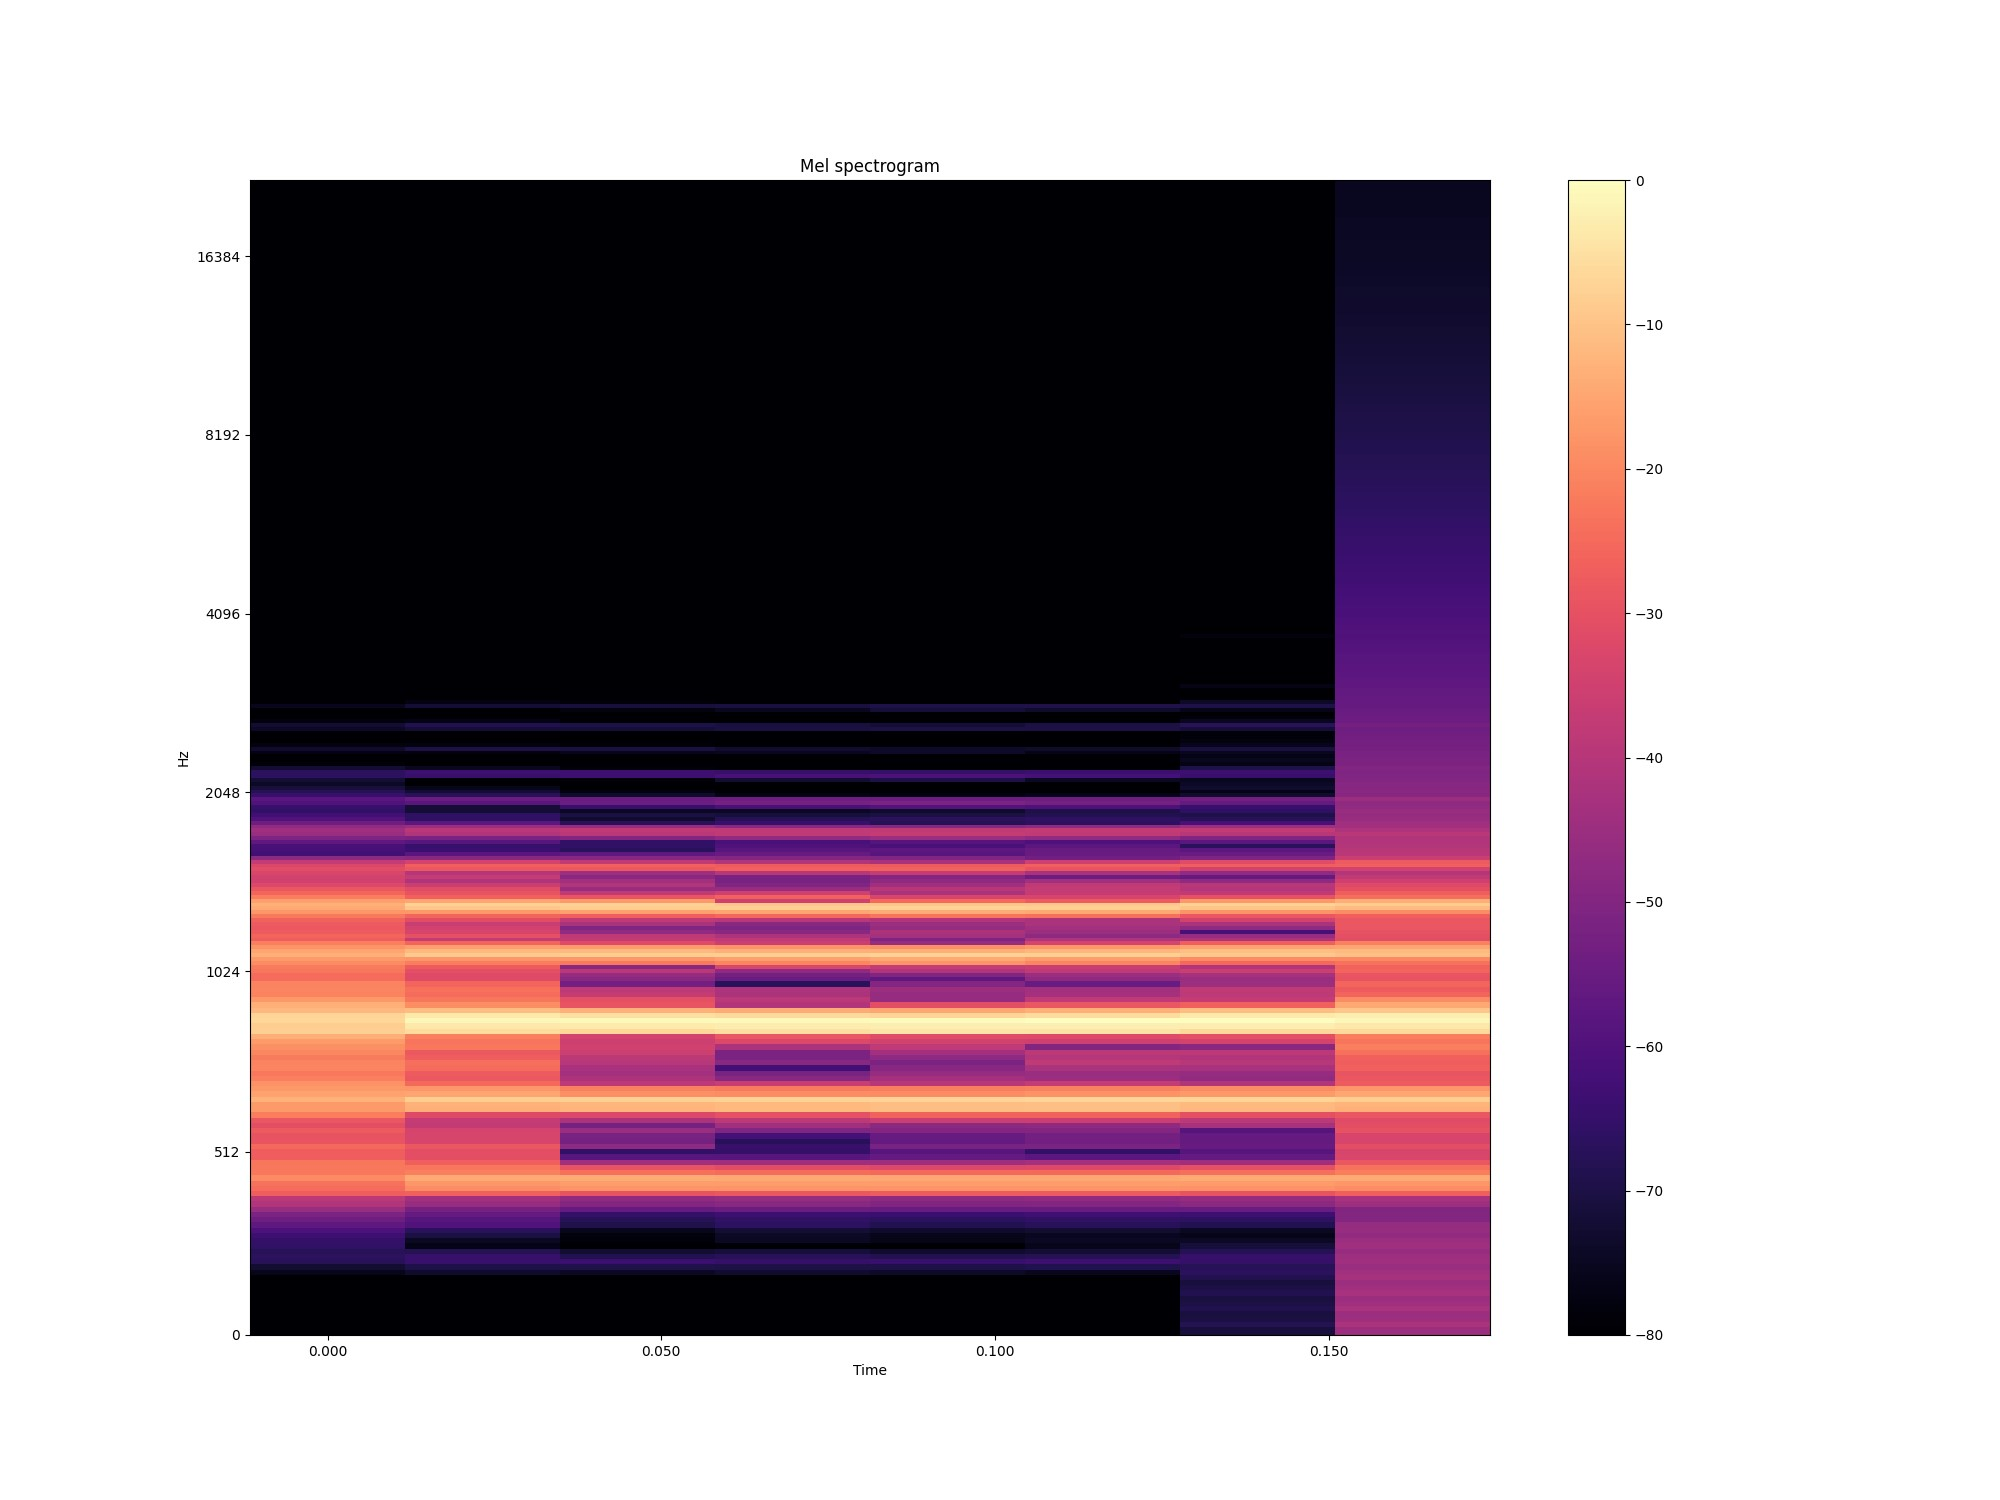
\includegraphics[width=\textwidth]{./img/spectrograms/HC_a}
        \caption{Przykładowy mel-spektrogram dla osoby zdrowej\@}
        \label{fig:melspectrogram_HC}
    \end{subfigure}
    \begin{subfigure}{0.49\textwidth}
        \centering
        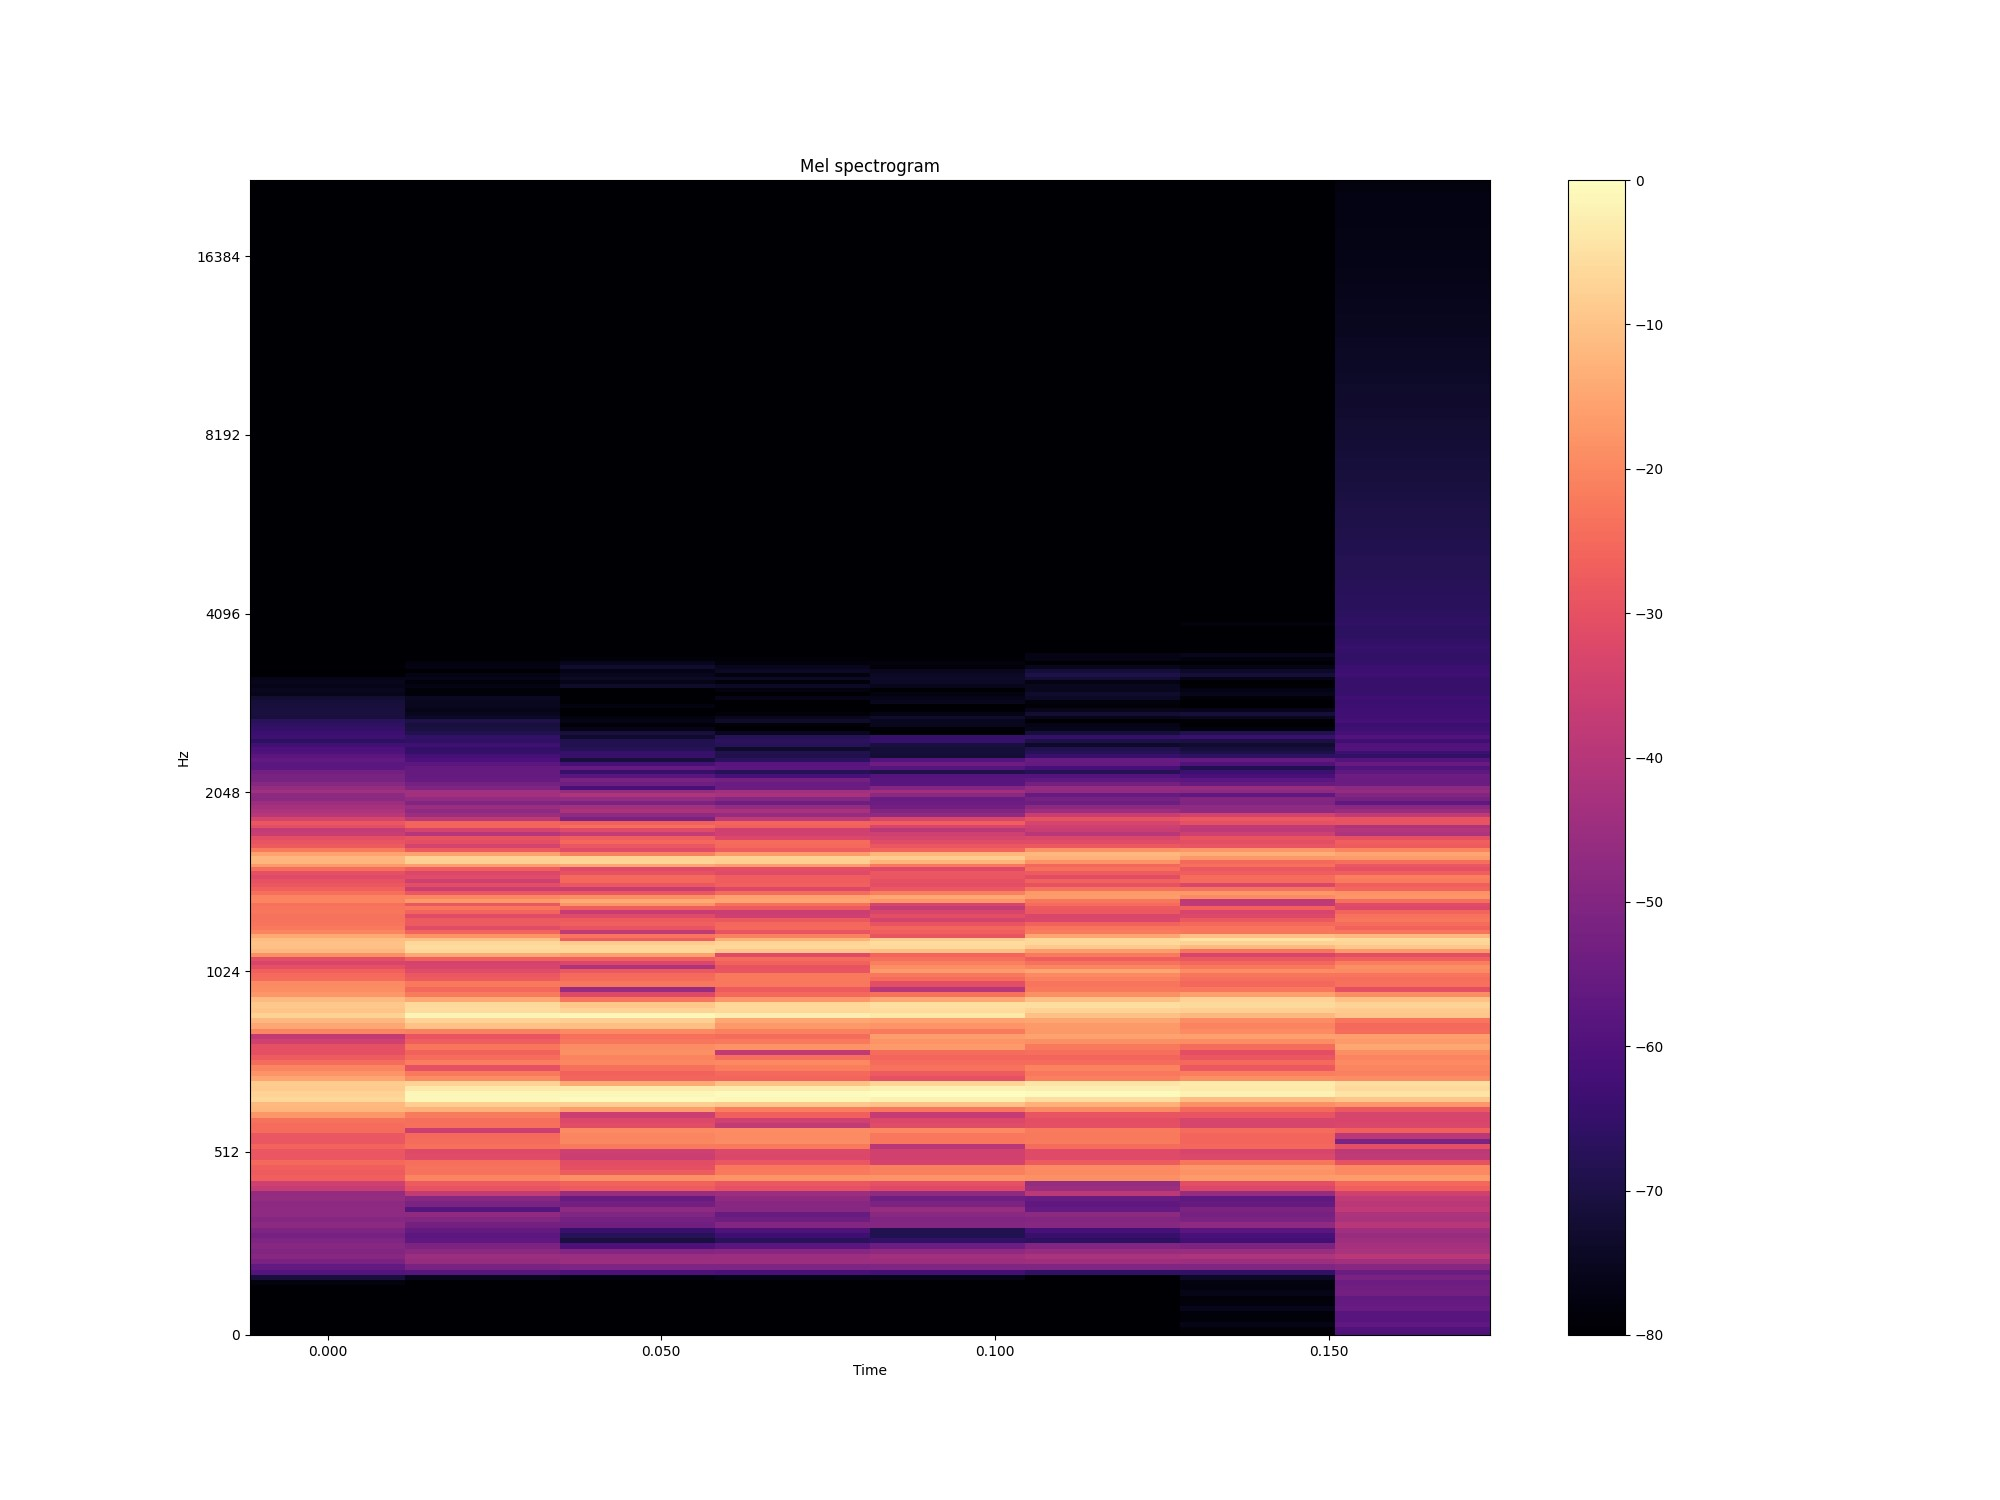
\includegraphics[width=\textwidth]{./img/spectrograms/PD_a}
        \caption{Przykładowy mel-spektrogram dla osoby z PD\@}
        \label{fig:melspectrogram_PD}
    \end{subfigure}

    \caption{Porównanie mel-spektrogramów osoby z PD oraz osoby zdrowej (hiszpańskojęzyczny zbiór danych, samogłoska /a/)}
    \label{fig:melspectrograms}
\end{figure}

Ważnym aspektem przy wyznaczaniu mel-spektrogramów są parametry takie jak liczba pasm Mel, rozmiar ramki analizy, długość przesunięcia (ang. \emph{overlap}) oraz rozdzielczość czasowa i częstotliwościowa.
Różne kombinacje tych parametrów mogą prowadzić do różnych szczegółów w reprezentacji dźwięku.
Wybór tych wartości został przeprowadzony na podstawie dostępną literaturę oraz własne eksperymenty.

Rozmiar okna czasowego jest jednym z kluczowych parametrów obliczeń melspektrogramów.
W kontekście diagnozowania choroby Parkinsona istnieje potrzeba uwzględnienia zarówno krótkotrwałych, dynamicznych zmian w mowie, jak i dłuższych charakterystyk.
Wybór długości okna (2048) został dokonany w celu uzyskania odpowiedniej rozdzielczości w dziedzinie czasu i częstotliwości, co pozwala na dokładniejsze odwzorowanie tych cech w mel-spektrogramie.
Długość przesunięcia określa, co ile próbek dźwiękowych nowe okno czasowe jest nakładane na sygnał.
W celu zachowania równowagi między dokładnością w dziedzinie czasu a efektywnością obliczeń wybrano \emph{hop\_length} o wartości 512.
Jest to kompromis, który pozwala na zachowanie informacji o krótkotrwałych zmianach w sygnale.
Liczba pasm Mel określa, ile pasm częstotliwościowych zostanie wygenerowanych w mel-spektrogramie.
W celu uzyskania szczegółowej reprezentacji widma dźwiękowego wybrano wartość równą 320.
Choroba Parkinsona może wprowadzać subtelne zmiany w mowie, dlatego ważne jest uwzględnienie wysokiej rozdzielczości w dziedzinie częstotliwości, co pozwala na dokładniejszą analizę sygnału mowy.


Często praktyką przed przekazaniem danych do sieci neuronowych (CNN) jest ich skalowanie.
Pomaga ono zapewnić zbieżność, stabilność i efektywność procesu uczenia się modelu, nie wprowadzając dodatkowych informacji.
Dlatego zdecydowano się na skalowanie metodą \emph{Min-Max}  na zakres od 0 do 1 opisaną wzorem~\eqref{eq:minmax}.

\begin{equation}
	\label{eq:minmax}
	X_{\text{scaled}} = \frac{X - X_{\min}}{X_{\max} - X_{\min}}
\end{equation}

\subsection{Augmentacja}
\label{subsec:augmentacja}

Aktualny stan wiedzy w dziedzinie automatycznej diagnostyki choroby Parkinsona ukazuje, że konwolucyjne sieci neuronowe (CNN) znacząco poprawiły wyniki w zadaniach przetwarzania mowy.
Jednakże, aby uniknąć przeuczenia, konieczna jest duża ilość danych treningowych.
Dostępne bazy danych zawierają zwykle do kilkuset nagrań, co ogranicza możliwość uwzględnienia wielu istotnych cech i stworzenia stabilnego modelu klasyfikacyjnego.

W początkowych eksperymentach przeprowadzonych w ramach tej pracy nie udało się osiągnąć oczekiwanych wyników, ze względu na bardzo duże przeuczenie (ang. \emph{overfitting}) testowanych modeli.
Jest to częsty problem, który można rozwiązać dzięki praktyce znanej jako augmentacja danych.
Polega ona na modyfikacji oryginalnych próbek, co prowadzi do zwiększenia ilości danych treningowych.
Augmentacja danych znacząco poprawia zdolność modeli CNN do generalizacji i zwiększa ich odporność na przeuczenie.

W badaniu opisanym w publikacji~\cite{augmentation} zastosowano sześć technik augmentacji danych specyficznych dla mowy w celu polepszenia zdolności modelu do generalizacji na dane, które nie były wcześniej widziane.
Wyniki tych badań pokazały, że wykorzystane techniki augmentacji  istotnie poprawiały zdolność do wykrywania zaburzeń mowy u pacjentów z chorobą Parkinsona.
Podobne znaczenie augmentacji danych jako istotnego czynnika wpływającego na skuteczność rozwiązań w dziedzinie klasyfikacji choroby Parkinsona podkreślono również w publikacji~\cite{Wodzinski}.

Dlatego w niniejszej pracy zdecydowano się zastosować 4 techniki augmentacyjne: przesunięcie w czasie, spowolnienie, przyspieszenie oraz losową zmianę wysokości dźwięku.
Wszystkie modyfikacje zostały przeprowadzone na sygnałach przed wyznaczeniem mel-spektrogramów.
Wpływ zmian na mel-spektrogramy przedstawiono na Rys~\ref{fig:augumentacja}.


\begin{enumerate}[label={\alph*)}]
	\item Przesunięcie w czasie (ang.~\emph{time shifting}). Dla zapewnienia, że model nie dostosowuje się do lokalizacji czasowej danej próbki mowy lub głosu, zmieniana jest kolejność sygnału.
Jest to osiągane poprzez przesunięcie sygnałów w prawo wzdłuż osi czasu o losową ilość, która jest mniejsza niż długość wejściowego nagrania audio.
    \item Losowa zmiana wysokości dźwięku (ang.~\emph{pitch change}). Składowe częstotliwości próbek są losowo przesuwane w dół lub w górę, przy czym należy zadbać o to, aby długość nie uległa zmianie poprzez rozciągnięcie oryginalnej próbki o losową ilość czasu z przedziału [3; 5] w dziedzinie czasu, a następnie jej resampling.
    \item Spowolnienie (ang.~\emph{slow-down}).
Przez rozciągnięcie w czasie próbki dźwiękowej zapewniamy, że model sieci neuronowej nie dostosowuje się tylko do prędkości mowy lub głosu badanego podmiotu.
Współczynnik spowolnienia jest losowo wybierany z przedziału [0,2; 0,8].
    \item Przyspieszenie (ang.~\emph{speed-up}). Tak samo, jak spowolnienie dźwięku, losowe przyspieszenie ma na celu zapobieganie dostosowywaniu modelu do prędkości mowy mówcy.
Współczynnik przyspieszenia jest losowo wybierany z przedziału [1,2; 2,5].
\end{enumerate}

Augmentacja została przeprowadzona tylko dla zbioru treningowego i walidacyjnego, aby zwiększyć różnorodność danych uczących oraz poprawić wydajność modelu w procesie uczenia maszynowego.
Zbiór testowy pozostaje nienaruszony, aby zachować jego niezmienność i umożliwić obiektywną ocenę skuteczności modelu na nieznanych wcześniej danych.

\begin{figure}[hp]
    \centering
    \begin{subfigure}{0.68\textwidth}
        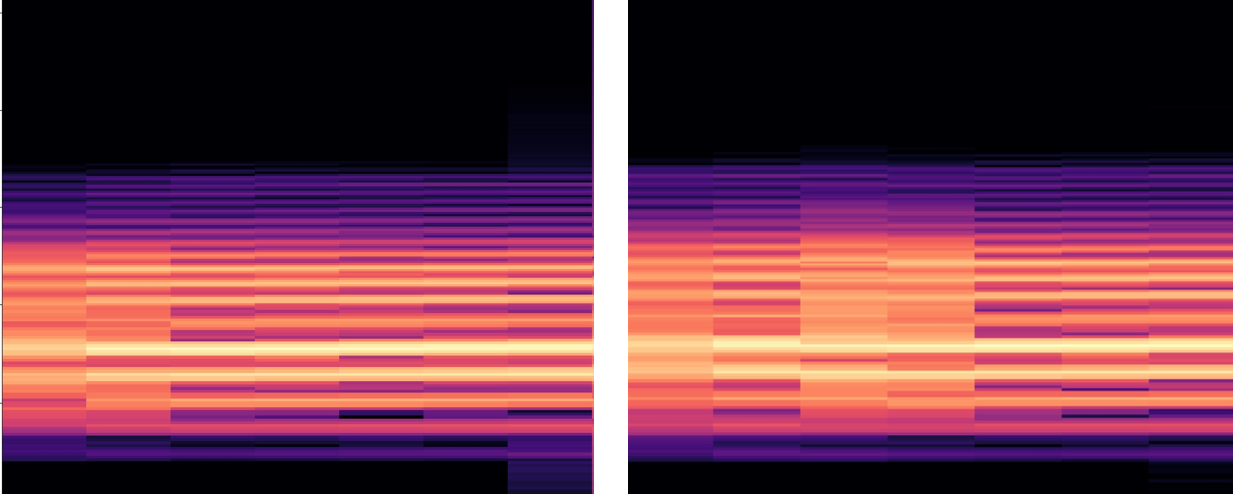
\includegraphics[width=\linewidth]{./img/augmentation/rolled}
        \caption{Przesunięcie w czasie\@}
        \label{fig:roll}
    \end{subfigure}

    \begin{subfigure}{0.68\textwidth}
        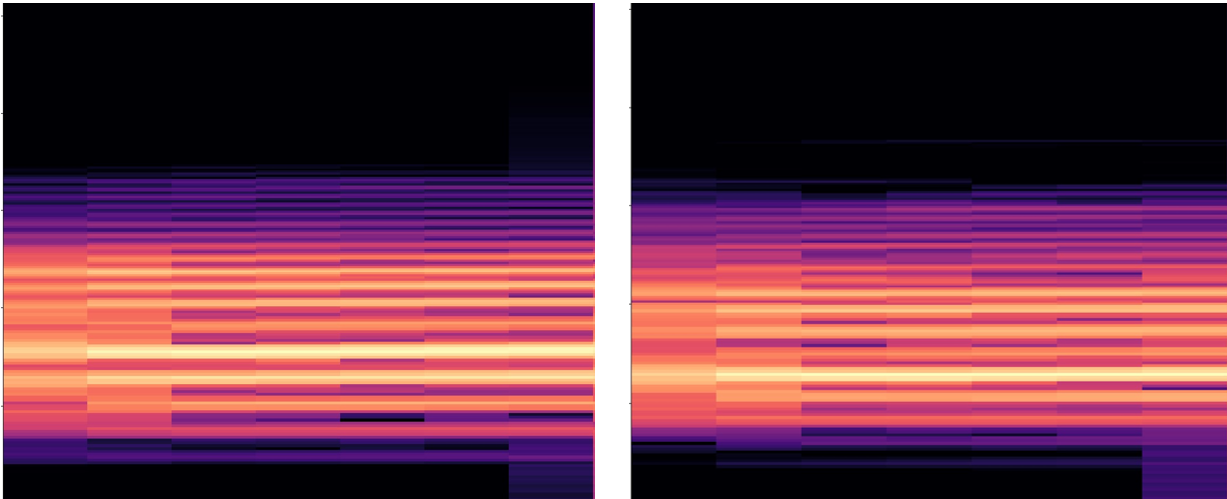
\includegraphics[width=\linewidth]{./img/augmentation/pitch}
        \caption{Zmiana wysokości dźwięku\@}
        \label{fig:pitch}
    \end{subfigure}

    \begin{subfigure}{0.68\textwidth}
        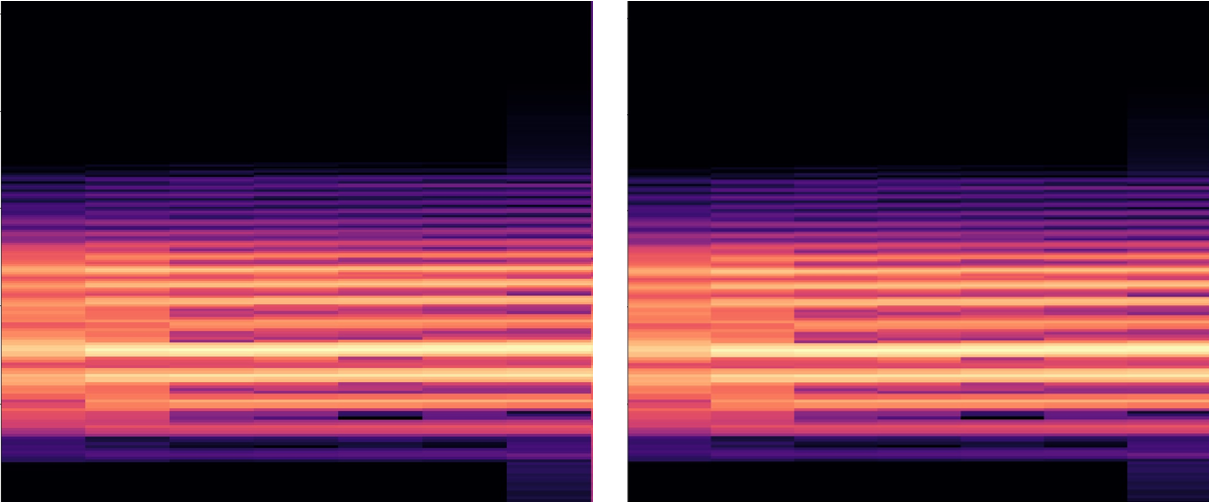
\includegraphics[width=\linewidth]{./img/augmentation/slow}
        \caption{Spowolnienie\@}
        \label{fig:slow}
    \end{subfigure}

    \begin{subfigure}{0.68\textwidth}
        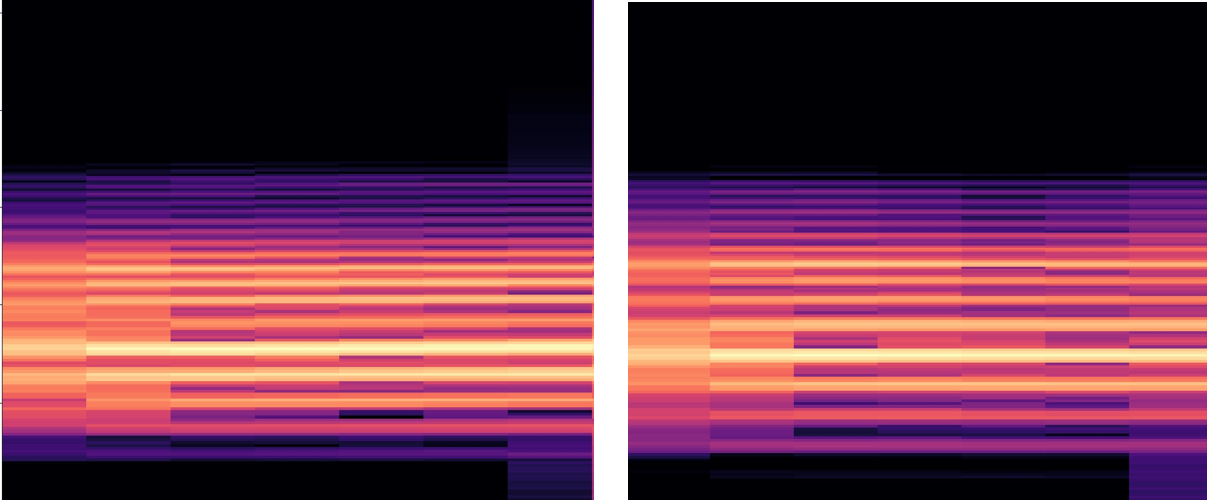
\includegraphics[width=\linewidth]{./img/augmentation/speed}
        \caption{Przyspieszenie\@}
        \label{fig:speed}
    \end{subfigure}

    \caption{Porównanie wpływu technik augmentacji na wygląd mel-spektrogramu. Po lewej stronie przedstawiony jest mel-spektrogram obliczony na podstawie surowego sygnału, a po prawej stronie widoczne są efekty augmentacji, w kolejności: (a) przesunięcie w czasie, (b) zmiana wysokości dźwięku, (c) spowolnienie sygnału oraz (d) przyspieszenie sygnału. (Zbiór danych: PC-GITA, samogłoska /a/, HC)}

    \label{fig:augumentacja}
\end{figure}

%---------------------------------------------------------------------------
%\newpage
\section{Metody klasyfikacji}
\label{sec:klasyfikacja}

Zdecydowano się na graficzne reprezentacje sygnałów, co wymaga też doboru odpowiednich metod klasyfikacji.
Popularnym rozwiązaniem są konwolucyjne sieci neuronowe (ang. \emph{Convolutional Neural Network}, CNN).
Jest to rodzaj zaawansowanych modeli uczenia maszynowego, które zostały pierwotnie zaprojektowane do przetwarzania i analizy danych wizualnych, takich jak obrazy i filmy.
Jednakże, ze względu na swoją skuteczność w ekstrakcji cech z danych przestrzennych, CNN znalazły zastosowanie także w dziedzinach związanych z przetwarzaniem dźwięku.

Główną cechą CNN są warstwy konwolucyjne.
Wykorzystują one filtry konwolucyjne, które przesuwają się po wejściowych danych, wyodrębniając lokalne wzorce, takie jak krawędzie, tekstury i inne cechy.
To pozwala na automatyczną ekstrakcję istotnych cech.
CNN często zawierają też warstwy \emph{pooling}, które zmniejszają rozmiar danych wyjściowych z warstw konwolucyjnych.
Pomaga to zmniejszyć liczbę parametrów w sieci i sprawia, że sieć jest bardziej odporna na przetwarzanie danych o różnych rozmiarach.
CNN zwykle składają się z wielu warstw konwolucyjnych i warstw \emph{fully connected}, które uczą się reprezentacji coraz bardziej abstrakcyjnych cech danych.
Są wysoce zdolne do rozpoznawania wzorców w danych, co czyni je skutecznymi w zadaniach klasyfikacji, detekcji obiektów, rozpoznawaniu mowy i wielu innych.
Dużą zaletą sieci konwolucyjnych jest możliwość skorzystania z uczenia z transferem, co oznacza wykorzystanie pretrenowanych modeli na dużych zbiorach danych, a następnie dostosowanie ich do konkretnej dziedziny lub zadania.

Konwolucyjne sieci neuronowe są potężnym narzędziem w analizie graficznych reprezentacji danych i są powszechnie stosowane w wielu dziedzinach, aby automatycznie ekstrahować i analizować cechy złożonych danych przestrzennych.
Dzięki ich zdolności do hierarchicznego uczenia się i rozpoznawania wzorców są używane w różnych zastosowaniach, w tym również w medycynie.
Dlatego zdecydowano się wykorzystać tę metodę do klasyfikacji mel-spektrogramów.

\subsection{Wykorzystane architektury}
\label{subsec:architektury}

Ze względu na ograniczoną dostępność danych głosowych pacjentów z chorobą Parkinsona, zastosowano technikę znaną jako \emph{transfer learning}.
Umożliwia ona wykorzystanie wstępnie wytrenowanych modeli, które zostały nauczane na dużym zbiorze danych,
do zadań diagnostycznych z wykorzystaniem ograniczonej ilości dostępnych danych głosowych.

Kluczowym krokiem było wybranie modeli, które miały dostępne wagi wytrenowane na dużym i takim samym zbiorze danych.
Zdecydowano się na ImageNet, ponieważ jest to jedna z najważniejszych baz danych obrazów wykorzystywana w dziedzinie komputerowego widzenia i uczenia maszynowego.
Wybrano modele takie jak Xception, MobileNetV2, InceptionV3, VGG16 i ResNet50.
Takie podejście pozwoliło na zaoszczędzenie czasu i zasobów, które byłyby potrzebne do wytrenowania sieci od podstaw na niewielkim zbiorze danych.
W ramach pracy magisterskiej skoncentrowano się na porównaniu różnych architektur w kontekście automatycznej diagnostyki choroby Parkinsona na podstawie analizy głosu.

\begin{enumerate}[label={\alph*)}]
    \item VGG16. To przykład klasycznego modelu CNN o głębokiej architekturze, opracowany przez Visual Geometry Group na Uniwersytecie Oksfordzkim.
    Jest znany ze swojej prostoty i skuteczności w ekstrakcji cech z obrazów.

    \item ResNet50. Jest to znana architektura CNN, która wprowadza innowacyjny pomysł na połączenia pomostowe, eliminujące problem znikającego gradientu w głębokich sieciach.
    Dzięki temu ResNet50 jest w stanie efektywnie uczyć się reprezentacji danych.

    \item Xception. Jest to model głębokiej nauki opracowany przez François Chollet w 2016 roku.
    Jest to jedna z odmian architektury konwolucyjnej sieci neuronowej (CNN), która wyróżnia się wyjątkową zdolnością do wykrywania cech hierarchicznych w obrazach.

    \item InceptionV3. Charakteryzuje się wykorzystaniem tzw. \emph{inception modules}, które pozwalają na efektywne wykrywanie wielu skal i rodzajów cech w obrazach.
    Został zaprojektowany przez Google.

    \item MobileNetV2. Jest to przykłąd lekkiej i efektywnej architektury CNN, zaprojektowanej z myślą o urządzeniach mobilnych
    Jej cechą charakterystyczną jest niska ilość parametrów i małe obliczenia, co sprawia, że jest idealna do zastosowań w zasobochłonnych zadaniach takich jak analiza głosu na urządzeniach mobilnych.

\end{enumerate}

Wybór tych konkretnych klasyfikatorów wynikał z różnorodności ich architektur i specjalizacji.
Choroba Parkinsona manifestuje się na różne sposoby w głosie pacjentów, dlatego zróżnicowane modele w różny sposób mogą wspomagać wydobycie istotnych cech.
Xception i InceptionV3 są znane z efektywności w ekstrakcji wielu rodzajów cech, co jest istotne przy analizie złożonych danych głosowych.
MobileNetV2, z kolei, jest lekki i mobilny, co pozwala na przenośność rozwiązania do urządzeń mobilnych, które mogą być używane w codziennym monitoringu pacjentów.
VGG16 i ResNet50, choć głębokie, mają zdolność do wyodrębniania skomplikowanych wzorców, co może być przydatne w diagnozie.
Porównanie różnych klasyfikatorów pozwoli na ocenę ich wydajności i skuteczności w diagnostyce na podstawie głosu.

Po początkowym przeszkoleniu na zbiorze danych ImageNet przeprowadzono proces \emph{fine-tuningu} na wcześniej przygotowanym zestawie danych.
Fine-tuning to technika dostosowywania już przeszkolonych modeli do specyficznych zastosowań.
Modele były dostosowywane w celu nauki rozpoznawania specyficznych cech akustycznych charakterystycznych dla pacjentów z chorobą Parkinsona.
Proces ten obejmował dodawanie dodatkowych warstw gęstych do modelu oraz wykorzystywanie techniki dropout, która pomaga uniknąć przeuczenia modelu.
Dzięki tym modyfikacjom klasyfikatory stały się bardziej odpowiednie do analizy dźwięku oraz diagnozowania choroby Parkinsona na podstawie danych głosowych

%W każdym przypadku wykorzystano pretrenowane wagi do ekstrakcji cech.
%Ostatnią warstwę gęstą zastąpiono odpowiednimi warstwami, zależnie od architektury sieci.
%Konfiguracje te zostały dobrane na podstawie zarówno dostępnej literatury, jak i własnych eksperymentów.

%W przypadku sieci VGG16  i InceptionV3 dodano jedną warstwę \emph{Dense} o rozmiarze 512 oraz warstwę Dropout o współczynniku 0,5.
%W ResNet50 oraz dodano warstwę dense o rozmiarze 128.
%W przypadku Xception podobnie jak w publikacji~\cite{augmentation}, dodano trzy warstwy dense o rozmiarze 128 oraz warstwę Dropout o współczynniku 0,5.
%W sieci MobileNetV2 dodano dwie warstwy dense o rozmiarze 128 oraz warstwę Dropout o współczynniku 0,5.
%Na koniec, do każdej z tych architektur dodaliśmy warstwę gęstą z dwoma neuronami i funkcją aktywacji~\emph{softmax}), aby umożliwić skuteczną klasyfikację.

\subsection{Dobór parametrów i optymalizacja modeli}
\label{subsec:optymalizacja-modeli}

Wszystkie eksperymenty przeprowadzono przy użyciu tych samych parametrów.
Testowano różne kombinacje, jednak te ustawienia okazały się optymalne dla badanego problemu.
W eksperymentach uwzględniono takie aspekty jak rozmiar partii (ang. \emph{batch-size}), funkcję  straty i optymalizator.

Wybór rozmiaru partii, czyli liczby próbek przetwarzanych jednocześnie przez sieć neuronową, ma znaczenie dla równowagi pomiędzy wydajnością obliczeniową a stabilnością procesu  uczenia.
Przyjęto rozmiar partii równy 32, co jest kompromisem między efektywnym wykorzystaniem zasobów obliczeniowych a stabilnością uczenia.

Funkcja straty, czyli binarna entropia krzyżowa, została wybrana ze względu na swoją skuteczność w problemach klasyfikacji binarnej.
Minimalizacja funkcji straty pozwala modelowi lepiej dopasować się do rzeczywistych klas i ocenić jakość predykcji sieci.
Ta metryka jest często stosowana w zadaniach klasyfikacji, ponieważ skupia się na porównywaniu prognozowanych klas z rzeczywistymi wartościami.

Wybór optymalizatora SGD (ang. \emph{Stochastic Gradient Descent}) był wynikiem eksperymentalnej analizy różnych algorytmów optymalizacji i ich właściwości.
Ponadto jest on najczęściej spotykany w literaturze dotyczącej tego problemu badawczego.
W każdej iteracji SGD losowo wybiera małe losowe podzbiory danych treningowych i oblicza gradient funkcji kosztu tylko na podstawie tych próbek, co pozwala na szybszą aktualizację wag modelu.
Ta stochastyczna natura SGD pomaga uniknąć utknięcia w minimach lokalnych.

Bardzo ważny w tym problemie klasyfikacyjnym jest odpowiedni dobór współczynnika uczenia (ang. \emph{learning rate}).
Wartość tego parametru wpływa na tempo, z jakim model aktualizuje swoje wagi podczas procesu uczenia.
Wysoki learning rate może prowadzić do oscylacji i trudności w zbieżności algorytmu, podczas gdy zbyt niski może spowolnić proces uczenia.
Dlatego optymalny wybór \emph{learning rate} jest istotnym krokiem w dostrojeniu algorytmu SGD do konkretnego problemu.
Zdecydowano się na ustawienie wartości współczynnika uczenia na 0,0005.

Modele były trenowane przez 50 epok, ponieważ zbyt duża liczba epok mogłaby prowadzić do przetrenowania na tak małej ilości danych, co wpłynęłoby negatywnie na ich zdolność do generalizacji na nowe dane.
Dodatkowo zastosowano monitorowanie funkcji straty.
Ten mechanizm umożliwia wczesne zatrzymanie treningu, jeśli funkcja straty przestaje się poprawiać przez określoną liczbę epok (w tym przypadku przyjęto 5).

\subsection{Podział danych}
\label{subsec:podzial-danych}

Klasyczną techniką w uczeniu maszynowym jest podział zbioru danych na 3 podzbiory: treningowy, testowy oraz walidacyjny.
W problemie klasyfikacji celem jest stworzenie algorytmu, który na podstawie znanych sobie, opisanych wzorców, będzie w stanie efektywnie rozpoznawać wzorce nieopisane i dotąd sobie nieznane.
Dlatego wydziela się zbiór treningowy, na podstawie którego model uczy się wzorców i dopasowuje do danych.
Aby uniknąć nadmiernego dopasowania danych do modelu (ang.
\emph{overfitting}) stosuje się również zbiór walidacyjny, który  przeprowadza bezstronną ocenę dopasowania modelu do zbioru danych szkoleniowych podczas dostrajania hiperparametrów modelu.
Na koniec ocenia się skuteczność modelu na niezależnym zbiorze testowym.

Inną często wykorzystywaną techniką jest wykorzystanie krosswalidacji (ang. \emph{cross-validation}).
Jest to technika oceny wydajności modelu maszynowego, która polega na podziale dostępnych danych na kilka części, z których jedna służy jako zbiór walidacyjny, a pozostałe jako zbiór treningowy.
Proces ten jest wielokrotnie powtarzany, aby uzyskać stabilniejszą ocenę wydajności modelu i uniknąć przeuczenia.
Najpopularniejszym typem krosswalidacji jest walidacja krzyżowa typu k-fold, gdzie dane są dzielone na k podzbiorów, a każdy z nich jest używany jako zbiór testowy w jednym z k cykli walidacji.

W pracy zastosowano 10-krotną walidację krzyżową oraz przyjęto podział na zbiór treningowy i testowy według proporcji 80:20 (biorąc pod uwagę osoby, nie liczbę nagrań).
Ważnym aspektem jest fakt, że podział nagrań dla różnych samogłosek przeprowadzono biorąc pod uwagę tożsamość mówcy (podejście \emph{subject-wise}).
To znaczy, że na przykład nagrania osoby, która znajduje się w zbiorze treningowym nie mogą wystąpić ani w testowym, ani walidacyjnym.
Ta zasada obowiązuje we wszystkich podzbiorach.
Pomaga to zachować spójne warunki uczenia i obiektywnie porównać otrzymane modele.
Nie dopuszcza to też możliwości, że model uczy się wzorców związanych z osobą, a nie chorobą Parkinsona.
Ostatecznie w zbiorze testowym znalazło się 90 nagrań od 30 osób.
W zbiorach walidacyjnym i treningowym liczby te nieco różniły się w różnych iteracjach krosswalidacji, ponieważ nie dla każdego mówcy dysponowano taką samą ilością nagrań.
Zbiór walidacyjny zawierał około 45 nagrań, a treningowy około 350.

%---------------------------------------------------------------------------

\section{Metody ewaluacji wyników}
\label{sec:metody-ewaluacji-wynikow}

W celu oceny skuteczności różnych metod klasyfikacji choroby Parkinsona przeprowadzono badania wykorzystujące różnorodne techniki ewaluacji.
Niniejsza sekcja zawiera prezentację wybranych metod, które zostały użyte w ramach przeprowadzonych eksperymentów.
Kluczowym aspektem jest konieczność zastosowania odpowiednich technik ewaluacji wyników.
Techniki te nie tylko umożliwiają obiektywną ocenę efektywności proponowanych rozwiązań, ale także pozwalają na porównanie ich ze sobą.
Dzięki temu pozwalają lepiej zrozumieć, które podejścia są najbardziej obiecujące w kontekście diagnozowania choroby Parkinsona i polepszania dokładności klasyfikacji, co jest kluczowe dla postępu w dziedzinie medycyny i diagnostyki tej choroby.

\subsection{Krzywe uczenia}
\label{subsec:krzywe-uczenia}

Krzywe uczenia są skutecznym narzędziem do wizualizacji procesu uczenia modelu.
W trakcie eksperymentów prowadzono monitorowanie dwóch kluczowych krzywych: dokładność (ang. \emph{accuracy}) i funkcję kosztu (ang. \emph{loss}).
Krzywa dokładności przedstawia zmiany dokładności modelu w trakcie treningu i walidacji, podczas gdy krzywa funkcji kosztu pokazuje, jak zmienia się funkcja kosztu w trakcie uczenia.
Analiza tych krzywych dostarcza istotnych informacji na temat efektywności uczenia modelu.
Pozwala ocenić, czy model uczy się poprawnie, czy może występują problemy z nadmiernym dopasowaniem  (ang. \emph{overfitting}) lub niedostatecznym dopasowaniem (ang. \emph{underfitting}).
Dzięki tym analizom można dokonać wniosków na temat jakości modelu i ewentualnie dostosować hiperparametry lub strategię treningową w celu uzyskania lepszych wyników.
Wartościowe informacje o procesie uczenia są kluczowe dla udanej implementacji modelu i oceny jego skuteczności.

\subsection{Metryki walidacyjne}
\label{subsec:metryki-waldiacyjne}

Podczas oceny skuteczności klasyfikacji, korzystano z najbardziej popularnych metryk, które pozwalają ocenić jakość predykcji modelu.
W podanych wzorach zastosowano oznaczenia:  TP – True Positive, TN – True Negative, FP – False Positive, FN – False Negative.

\begin{enumerate}[label={\alph*)}]
    \item Błędy I i II rodzaju
    \item [] Jest to popularne narzędzie służące do analizy wyników klasyfikacji.
    Błąd I rodzaju (ang. \emph{False Positive}) oznacza błędną klasyfikację przypadku, który jest negatywny, jako pozytywny.
    W kontekście Parkinsona oznacza to, że model zaklasyfikował zdrową osobę jako chorą na chorobę Parkinsona.
    Błąd II rodzaju (ang. \emph{False Negative}) oznacza błędną klasyfikację przypadku, który jest pozytywny, jako negatywny.
    W kontekście Parkinsona oznacza to, że model zaklasyfikował osobę chorą na chorobę Parkinsona jako zdrową.

    \item [] Analiza błędów I i II rodzaju ma duże znaczenie w kontekście ewaluacji systemów diagnostycznych.
    Błąd I rzędu może prowadzić do niezdiagnozowania choroby u pacjenta, podczas gdy błąd II rzędu może prowadzić do błędnego zdiagnozowania osoby zdrowej jako cierpiącej na chorobę Parkinsona.
    Ważne jest, aby oceniać i minimalizować te błędy w celu uzyskania jak najdokładniejszej klasyfikacji.

    \item [] W systemach diagnostycznych większe znaczenie ma minimalizacja błędów II rodzaju.
    W przypadku wykorzystania takiego narzędzia jako wspomagającego proces diagnozy zaklasyfikowanie osoby zdrowej jako chorej spowoduje jedynie dalszą diagnostykę.
    Natomiast jeśli osoba chora rozpoznana zostanie jako zdrowa, proces jej leczenia rozpocznie się później, co może przynieść różne skutki.
	\item Dokładność (ang.~\emph{accuracy})
    \item [] To prosta i intuicyjna miara, która oblicza stosunek poprawnie sklasyfikowanych próbek do wszystkich próbek.
    Wyraża ona ogólną skuteczność klasyfikacji.
    Opisywana jest wzorem~\ref{eq:accuracy}
    \begin{equation}
        \text{Accuracy} = \frac{TP + TN}{TP + FN + TN + FP}
        \label{eq:accuracy}
    \end{equation}
    , gdzie:

\quad$TP$ - True Positives (prawdziwie pozytywne),

\quad$TN$ - True Negatives (prawdziwie negatywne),

\quad$FP$ - False Positives (fałszywie pozytywne),

\quad$FN$ - False Negatives (fałszywie negatywne).

    \item Precyzja (ang.~\emph{precision})
    \item [] Mierzy stosunek prawdziwie pozytywnych predykcji do sumy prawdziwie pozytywnych i  fałszywie pozytywnych predykcji.
Wyraża zdolność modelu do identyfikowania prawdziwie pozytywnych przypadków.
Określa się ją wzorem~\ref{eq:precision}
      \begin{equation}
        \text{Precision} = \frac{TP}{TP + FP}\label{eq:precision}
    \end{equation}
    , gdzie:

\quad$TP$ - True Positives (prawdziwie pozytywne),

\quad$FP$ - False Positives (fałszywie pozytywne).

    \item Czułość (ang.~\emph{recall})
    \item [] Jest to stosunek prawdziwie pozytywnych predykcji do sumy prawdziwie pozytywnych i fałszywie negatywnych predykcji.
Wyrażana jest wzorem~\ref{eq:recall} i określa zdolność modelu do wykrywania wszystkich prawdziwie pozytywnych przypadków.
    \begin{equation}
        \text{Recall} = \frac{TP}{TP + FN}\label{eq:recall}
    \end{equation}
    , gdzie:

\quad$TP$ - True Positives (prawdziwie pozytywne),

\quad$FN$ - False Negatives (fałszywie negatywne).

    \item Miara F1 (ang.~\emph{F1-score})
    \item [] To harmoniczna średnia precyzji i czułości.
Jest używana jako miara równowagi między precyzją a czułością.
Wyższe wartości wskazują na lepszą jakość klasyfikacji modelu.
Wyraża się ją wzorem~\ref{eq:f1}.
  \begin{equation}
        \text{F1} = \frac{2 * TP}{2 * TP + FP + FN}\label{eq:f1}
    \end{equation}
        , gdzie:

\quad$TP$ - True Positives (prawdziwie pozytywne),

\quad$FP$ - False Positives (fałszywie pozytywne),

\quad$FN$ - False Negatives (fałszywie negatywne).

\end{enumerate}
\chapter{Wyniki badań}

\section{Samogłoska /a/}
\label{sec:samogloska-a}

%---------------------------------------------------------------------------

\section{Samogłoska /e/}
\label{sec:samogloska-e}

%---------------------------------------------------------------------------

\section{Samogłoska /i/}
\label{sec:samogloska-i}

%---------------------------------------------------------------------------

\section{Samogłoska /o/}
\label{sec:samogloska-o}

%---------------------------------------------------------------------------

\section{Samogłoska /u/}
\label{sec:samogloska-u}

%---------------------------------------------------------------------------

\section{Zbiorcze podsumowanie wyników}
\label{sec:podsumowanie-wynikow}
\chapter{Analiza i interpretacja wyników}



Komputerowe wykrywanie choroby Parkinsona umożliwi przesiewowe badania populacji oraz częste monitorowanie, dostarczając bardziej obiektywny pomiar objawów, co przyniesie korzyści zarówno pacjentom, jak i dostawcom opieki zdrowotnej.
\chapter{Podsumowanie}





%Kod poniżej dodaje Bibliografię do spisu treści
\cleardoublepage{}
\phantomsection{}
\addcontentsline{toc}{chapter}{Bibliografia}
\printbibliography{}


% itd.
% \appendix
% \include{dodatekA}
% \include{dodatekB}
% itd.

%\printbibliography{}

\end{document}
